% RG-TTA: Regime-Guided Meta-Control for Test-Time Adaptation in Streaming Time Series
% Adapt author names and affiliations before submission.
\documentclass[journal]{IEEEtran}

% --- Core packages ---
\usepackage[utf8]{inputenc}
\usepackage[T1]{fontenc}
\usepackage{amsmath,amssymb,amsthm}
\usepackage{graphicx}
\usepackage{booktabs}
\usepackage[hyphens]{url}    % allow URL line breaks at hyphens (before hyperref)
\usepackage[breaklinks=true,hidelinks,hypertexnames=false]{hyperref}
\usepackage{cite}            % IEEE-style citations (replaces natbib)
\usepackage{xcolor}
\usepackage{multirow}
\usepackage{enumitem}
\usepackage{algorithm}
\usepackage{algorithmic}
\usepackage[section]{placeins}
\usepackage{stfloats}        % enable bottom-of-page full-width floats
\usepackage{microtype}       % improved line breaking and character protrusion

% --- Widow/orphan control ---
\widowpenalty=10000
\clubpenalty=10000
\displaywidowpenalty=10000

% --- Float placement tuning (accommodate many tables/figures) ---
\renewcommand{\topfraction}{0.9}
\renewcommand{\bottomfraction}{0.9}
\renewcommand{\textfraction}{0.1}
\renewcommand{\floatpagefraction}{0.8}
\renewcommand{\dbltopfraction}{0.9}
\renewcommand{\dblfloatpagefraction}{0.8}
\setcounter{topnumber}{4}
\setcounter{bottomnumber}{4}
\setcounter{totalnumber}{8}
\setcounter{dbltopnumber}{4}

% --- Theorem environments (IEEEtran-compatible) ---
\newtheorem{proposition}{Proposition}
\newtheorem{theorem}{Theorem}
\newtheorem{corollary}{Corollary}
\newtheorem{definition}{Definition}

% --- IEEEtran proof environment fix ---
\renewenvironment{proof}[1][Proof]{\noindent\textit{#1.}\space}{\hfill$\blacksquare$\par\medskip}

% Repository
\newcommand{\repourl}{\url{https://github.com/IndarKarhana/RGTTA-Regime-Guided-Test-Time-Adaptation}}

\begin{document}

\title{RG-TTA: Regime-Guided Meta-Control for Test-Time Adaptation in Streaming Time Series}

\author{Indar~Kumar,
Akanksha~Tiwari,
Sai~Krishna~Jasti,
and~Ankit~Hemant~Lade%
\thanks{Code and data are available at \repourl.}%
\thanks{I.~Kumar, A.~Tiwari, S.~K.~Jasti, and A.~H.~Lade are independent researchers
(e-mail: indarkarhana@gmail.com, akankshat2803@gmail.com,
jsaikrishna379@gmail.com, ankitlade12@gmail.com).}}

\maketitle

% ============================================================
\begin{abstract}
% ============================================================

Test-time adaptation (TTA) enables neural forecasters to adapt to distribution shifts in streaming time series, but existing methods apply the same adaptation intensity regardless of the nature of the shift. We propose \textbf{Regime-Guided Test-Time Adaptation (RG-TTA)}, a meta-controller that \emph{continuously modulates} adaptation intensity based on distributional similarity to previously-seen regimes. Using an ensemble of Kolmogorov--Smirnov, Wasserstein-1, feature-distance, and variance-ratio metrics, RG-TTA computes a similarity score for each incoming batch and uses it to (i)~smoothly scale the learning rate---more aggressive for novel distributions, conservative for familiar ones---and (ii)~control gradient effort via loss-driven early stopping rather than fixed budgets, allowing the system to allocate exactly the effort each batch requires. As a supplementary mechanism, RG-TTA gates checkpoint reuse from a regime memory, loading stored specialist models only when they demonstrably outperform the current model (loss improvement $\geq$30\%).

RG-TTA is \emph{model-agnostic} and \emph{strategy-composable}: it wraps any forecaster exposing \texttt{train/predict/save/load} interfaces and enhances any gradient-based TTA method. We demonstrate three compositions---RG-TTA, RG-EWC, and RG-DynaTTA---and evaluate 6 update policies (3~baselines + 3~regime-guided variants) across 4 compact architectures (GRU, iTransformer, PatchTST, DLinear), 14 datasets (6~real-world multivariate benchmarks + 8~synthetic regime scenarios), and 4 forecast horizons (96, 192, 336, 720) under a streaming evaluation protocol with 3 random seeds (672 experiments total).

Regime-guided policies achieve the lowest MSE in \textbf{156 of 224} seed-averaged experiments (\textbf{69.6\%}), with RG-EWC winning 30.4\% and RG-TTA winning 29.0\%. Overall, RG-TTA reduces MSE by 5.7\% vs TTA while running 5.5\% faster; RG-EWC reduces MSE by 14.1\% vs standalone EWC. Against full retraining (672 additional experiments, 3 architectures excluding DLinear), RG policies achieve a median 27\% MSE reduction while running 15--30$\times$ faster, winning 71\% of seed-averaged configurations. The regime-guidance layer composes naturally with existing TTA methods, improving accuracy without modifying the underlying forecaster.

\end{abstract}

% ============================================================
\section{Introduction}
\label{sec:intro}
% ============================================================

Time series forecasting in production is inherently incremental: data arrives in batches, and the system must decide how to update its model~\cite{lim2021timeseries,benidis2023deep}. Test-time adaptation (TTA)~\cite{liang2024tta} has emerged as a practical approach, applying a fixed number of gradient steps to each incoming batch. Recent work has improved upon fixed TTA: TAFAS~\cite{kim2025tafas} freezes the source model and learns calibration modules (GCMs) that adapt predictions, while DynaTTA~\cite{grover2025dynatta} dynamically adjusts the learning rate based on prediction-error z-scores and embedding drift.

However, DynaTTA (and similar reactive methods) \emph{react} to current performance signals without asking the \emph{proactive} question: \textit{has the system seen this distribution before?} If a previously-encountered regime recurs, the highest-accuracy strategy is to load the checkpoint trained for that regime---not to re-adapt from a potentially stale model, which wastes gradient budget re-learning patterns that were already captured.

We propose \textbf{Regime-Guided Test-Time Adaptation (RG-TTA)}, a meta-controller that adds this proactive layer. For each incoming batch, RG-TTA:
\begin{enumerate}[nosep]
  \item Extracts a 5-dimensional distributional feature vector (mean, std, skewness, excess kurtosis, lag-1 autocorrelation).
  \item Computes similarity to all stored regime checkpoints using an ensemble of Kolmogorov--Smirnov, Wasserstein-1, feature-distance, and variance-ratio metrics.
  \item Uses the similarity score to \emph{continuously} modulate adaptation:
  \begin{itemize}[nosep]
    \item \textbf{Learning rate} scales smoothly with novelty: $\alpha = \alpha_{\text{base}} \cdot (1 + \gamma \cdot (1 - \text{sim}))$, where $\gamma = 0.67$.
    \item \textbf{Checkpoint reuse} is loss-gated: stored checkpoints are loaded only when $\text{sim} \geq 0.75$ \emph{and} the checkpoint's loss is $< 0.70 \times$ the current model's loss ($\geq$30\% improvement).
    \item \textbf{Step count} is determined by loss-driven early stopping (patience $= 3$, $\epsilon = 0.005$), up to a maximum of 25 steps.
  \end{itemize}
\end{enumerate}

RG-TTA is \emph{model-agnostic}: it requires only \texttt{train()}, \texttt{predict()}, and \texttt{save/load\_weights()} interfaces and can wrap any forecaster. It is also \emph{strategy-composable}: the regime-guidance layer can enhance any gradient-based adaptation method (TTA, EWC, DynaTTA), yielding RG-TTA, RG-EWC, and RG-DynaTTA variants.

Our contributions are:
\begin{enumerate}[nosep]
  \item A \textbf{continuous regime-guided adaptation policy} that modulates learning rate, step budget, and checkpoint reuse based on distributional similarity, using an ensemble of four complementary similarity metrics and loss-driven early stopping.
  \item A \textbf{composable meta-controller architecture} where regime-guidance wraps gradient-based adaptation methods, demonstrated with three compositions (RG-TTA, RG-EWC, RG-DynaTTA) targeting different accuracy--robustness trade-offs.
  \item A \textbf{comprehensive benchmark} spanning 6 update policies (plus full retraining), 4 compact model architectures, 14 datasets, 4 forecast horizons, and 3 random seeds (672 experiments, plus 672 retrain-baseline experiments)---to our knowledge, the most extensive controlled comparison of TTA strategies for streaming time series forecasting.
\end{enumerate}


% ============================================================
\section{Related Work}
\label{sec:related}
% ============================================================

\paragraph{Test-time adaptation for time series.}
TTA~\cite{liang2024tta} adapts a pre-trained model to test-time distribution shifts by running additional gradient steps. In the time series setting, TAFAS~\cite{kim2025tafas} proposes freezing the source model and training lightweight \emph{Gated Calibration Modules} (GCMs) that adjust inputs and outputs to the current distribution, using only pseudo-labels from the model's own predictions (POGT loss). DynaTTA~\cite{grover2025dynatta} extends TAFAS with a dynamic learning rate computed via a sigmoid transformation of three shift metrics: prediction-error z-score, and distances to recent (RTAB) and representative (RDB) embedding buffers. Both methods are \emph{reactive}---they adjust to the current batch based on real-time error and drift signals. RG-TTA adds a \emph{proactive} layer: it identifies whether the current distribution has been seen before and adapts its strategy accordingly. RG-TTA composes naturally with DynaTTA (RG-DynaTTA); we demonstrate this as a two-level controller.

\textbf{Reimplementation note.} DynaTTA's official codebase (\texttt{shivam-grover/DynaTTA}) implements the dynamic learning rate \emph{within} the TAFAS framework---tightly coupled with GCM calibration modules, the POGT pseudo-label loss, and a sliding-window evaluation harness. No standalone library or modular API is provided. Because our study requires a model-agnostic streaming evaluation pipeline that applies each update policy to the same frozen-backbone base model, we reimplemented DynaTTA's Algorithm~1 (dynamic LR via sigmoid of prediction-error z-score, RTAB/RDB embedding distances, and EMA smoothing) from the published description. Our implementation reproduces the published formula exactly with the published hyperparameters ($\alpha_{\min}=10^{-4}$, $\alpha_{\max}=10^{-3}$, $\kappa=1.0$, $\eta=0.1$). We validate on the same architectures targeted by DynaTTA (iTransformer, PatchTST). We note that DynaTTA's EMA coefficient ($\eta=0.1$) requires $\sim$22 gradient steps to converge, a design choice suited to the 500-window sliding-window protocol used in its original evaluation. Under our streaming protocol (10 batches per run), the EMA does not converge within the available budget, leaving the dynamic LR below TTA's fixed rate for the first 5--6 batches. This is a \emph{protocol-level mismatch}, not an implementation error (see Limitations~\S\ref{sec:limitations}, item~7).

TAFAS~\cite{kim2025tafas} is a strong baseline at short horizons (H$\leq$192) where its frozen-source GCM calibration excels, but its performance collapses at longer horizons (H=336/720, $+$100--400\% vs TTA in our experiments)---a consequence of its design for sliding-window evaluation. Because our study spans H$\in$\{96,192,336,720\}, we include TAFAS as a reference policy but exclude it from the primary 6-policy comparison.

\paragraph{Continual learning and catastrophic forgetting.}
Continual learning~\cite{parisi2019continual,mccloskey1989catastrophic} addresses the problem of updating a model on sequential tasks without forgetting old knowledge. EWC~\cite{kirkpatrick2017ewc} penalises changes to parameters important for previous tasks via the diagonal Fisher Information Matrix. Synaptic Intelligence~\cite{zenke2017continual} tracks parameter importance online. Experience replay~\cite{rolnick2019experience} stores and re-uses past data samples. Progressive networks~\cite{rusu2016progressive} add capacity for new tasks. Our approach is complementary: rather than regularising a single model, RG-TTA maintains a \emph{library of checkpoints} indexed by distributional features and selects the appropriate one. When combined with EWC (RG-EWC), the regime-guided adaptation operates under EWC regularisation ($\lambda = 400$), preventing catastrophic forgetting while benefiting from checkpoint reuse and similarity-modulated learning rates.

\paragraph{Concept drift and regime switching.}
Concept drift detection~\cite{gama2014concept,lu2018concept,aminikhanghahi2017survey} identifies \emph{that} a distribution change occurred. Our approach extends this by detecting not just \emph{change} but \emph{recurrence}---whether the new distribution matches a previously-seen regime. Hamilton's Markov-switching model~\cite{hamilton1989} uses latent states for regime transitions but assumes a specific generative process. RG-TTA makes no parametric assumption: ``regime'' is defined operationally by a 5-dimensional distributional feature vector, and matching uses non-parametric statistical tests.

\paragraph{Time series forecasting architectures.}
Recent neural forecasters---Informer~\cite{zhou2021informer}, Autoformer~\cite{wu2021autoformer}, iTransformer~\cite{liu2024itransformer}, PatchTST~\cite{nie2023patchtst}, DLinear~\cite{zeng2023dlinear}---advance accuracy but do not address the \emph{when-to-adapt} question. We evaluate RG-TTA across four compact model architectures spanning three model families---recurrent (GRU~\cite{cho2014gru}), attention-based (iTransformer, PatchTST), and linear (DLinear)---to validate model-agnosticism. Notably, iTransformer and PatchTST are the same modern Transformer architectures targeted by DynaTTA~\cite{grover2025dynatta}.


% ============================================================
\section{Method}
\label{sec:method}
% ============================================================

Figure~\ref{fig:workflow} provides an end-to-end overview of the RG-TTA pipeline; its main components---distributional similarity (\S\ref{sec:similarity}), continuous regime-guided adaptation (\S\ref{sec:adaptation}), and checkpoint management (\S\ref{sec:checkpoints})---are detailed in the subsections below.

\begin{figure*}[t]
\centering
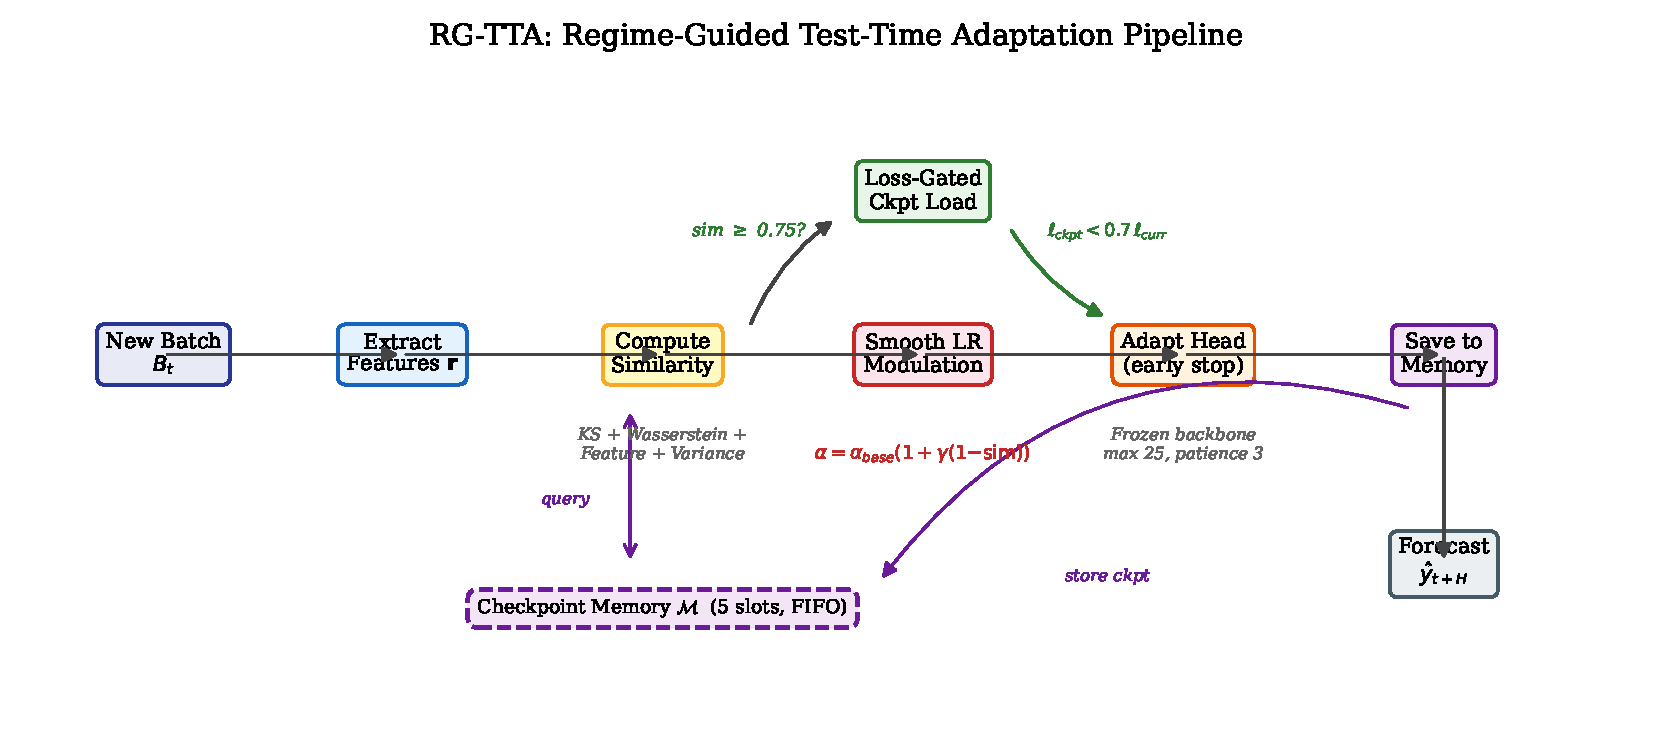
\includegraphics[width=0.95\textwidth]{figures/workflow.pdf}
\caption{RG-TTA system overview. For each incoming batch~$B_t$, the system extracts a distributional feature vector~$\mathbf{r}$ (Eq.~\ref{eq:features}) and computes a similarity score~$\text{sim}$ against stored regimes using a four-metric ensemble (Eq.~\ref{eq:ensemble}). If a high-similarity checkpoint passes the loss gate ($\ell_{\text{ckpt}} < 0.70\,\ell_{\text{curr}}$, Eq.~\ref{eq:gate}), it replaces the current model. The learning rate is smoothly modulated by similarity (Eq.~\ref{eq:lr}), and the output head is adapted with loss-driven early stopping (max~25 steps, patience~3). The adapted checkpoint and its regime features are stored in the memory~$\mathcal{M}$ (dashed box; 5~slots, FIFO eviction) for future reuse. See Algorithm~\ref{alg:rgtta} for pseudocode.}
\label{fig:workflow}
\end{figure*}

\subsection{Problem Setup}

Data arrives as a stream of batches $B_1, B_2, \ldots$ (batch size 750). A base forecaster $f_\theta$ can be trained, saved, and loaded. At each step $t$, batch $B_t$ arrives; the system produces a forecast $\hat{y}_{t+1:t+H}$ for horizon $H \in \{96, 192, 336, 720\}$ and optionally updates $\theta$. All 6 compared policies share the same $f_\theta$ architecture, the same data splits, and the same random seeds; only the update rule differs.

\subsection{Distributional Similarity Metric}
\label{sec:similarity}

For each batch, RG-TTA extracts a 5-dimensional distributional feature vector:
\begin{equation}
  \mathbf{r} = \big(\mu,\; \sigma,\; \gamma_1,\; \kappa{-}3,\; r_1\big),
  \label{eq:features}
\end{equation}
where $\mu$ is the mean, $\sigma$ the standard deviation, $\gamma_1$ the skewness, $\kappa{-}3$ the excess kurtosis, and $r_1$ the lag-1 autocorrelation. These features are computed from the most recent $3 \times \text{season\_length}$ samples of the target series and capture the distribution's location, scale, shape, tail behaviour, and temporal structure in $O(n)$ time. The deliberate simplicity of this feature vector is a design choice, not a limitation: it is cheap to compute (adding $<$0.1\% latency), fully interpretable, and---as the 69.6\% win rate across 14 diverse datasets confirms---\emph{sufficient} for effective regime discrimination. Richer representations (e.g., learned embeddings or spectral features) could capture more complex regime structures, but at the cost of additional parameters, training overhead, and opacity.

Similarity between a query batch $\mathbf{q}$ and a stored regime $\mathbf{s}$ is computed as a weighted ensemble of four complementary metrics:

\paragraph{Kolmogorov--Smirnov similarity.} Based on the two-sample KS statistic~\cite{massey1951ks} on the raw values:
\begin{equation}
  \text{sim}_{\text{KS}} = 1 - D_n, \quad D_n = \sup_x |F_{\mathbf{q}}(x) - F_{\mathbf{s}}(x)|.
\end{equation}

\paragraph{Wasserstein-1 similarity.} Normalised earth-mover's distance~\cite{villani2009optimal}:
\begin{equation}
  \text{sim}_{\text{W}} = \frac{1}{1 + W_1(\mathbf{q}_{\text{raw}}, \mathbf{s}_{\text{raw}}) \,/\, \max(\text{ptp}(\mathbf{q}_{\text{raw}}), \text{ptp}(\mathbf{s}_{\text{raw}}), \epsilon)}.
\end{equation}

\paragraph{Feature-distance similarity.} Normalised Euclidean distance in feature space:
\begin{equation}
  \text{sim}_{\text{feat}} = \frac{1}{1 + \|\mathbf{q} - \mathbf{s}\|_2 \,/\, \big((\|\mathbf{q}\|_2 + \|\mathbf{s}\|_2)/2 + \epsilon\big)}.
\end{equation}

\paragraph{Variance-ratio similarity.} Captures volatility regime shifts:
\begin{equation}
  \text{sim}_{\text{var}} = \frac{\min(\sigma_{\mathbf{q}}, \sigma_{\mathbf{s}})}{\max(\sigma_{\mathbf{q}}, \sigma_{\mathbf{s}}) + \epsilon}.
\end{equation}

\paragraph{Weighted ensemble.}
\begin{equation}
  \text{sim}(\mathbf{q}, \mathbf{s}) = 0.3 \cdot \text{sim}_{\text{KS}} + 0.3 \cdot \text{sim}_{\text{W}} + 0.2 \cdot \text{sim}_{\text{feat}} + 0.2 \cdot \text{sim}_{\text{var}}.
  \label{eq:ensemble}
\end{equation}
The statistical tests (KS, Wasserstein) use the full empirical distribution and receive higher weight (0.3 each) because they are non-parametric and distribution-free, capturing arbitrary shape differences that scalar features may miss. The feature-distance and variance-ratio metrics receive lower weight (0.2 each) as they provide complementary but narrower information (higher-order moments and volatility regime shifts, respectively). We chose these weights a priori based on the principle of giving distributional tests priority over scalar summaries, and did not tune them on validation data. The ablation in Table~\ref{tab:sim_ablation} confirms the ensemble is robust: it outperforms every single-metric variant, and the 1.8\% gap to the best single component (Wasserstein) suggests the ensemble's value lies in complementary coverage rather than precise weight selection.

\subsection{Continuous Regime-Guided Adaptation}
\label{sec:adaptation}

Rather than discretising similarity into fixed tiers with predetermined step counts, RG-TTA uses the similarity score as a \emph{continuous} control signal for three adaptation dimensions:

\paragraph{Smooth learning rate modulation.} The learning rate scales smoothly with distributional novelty:
\begin{equation}
  \alpha = \alpha_{\text{base}} \cdot \big(1 + \gamma \cdot (1 - \text{sim})\big),
  \label{eq:lr}
\end{equation}
where $\alpha_{\text{base}} = 3 \times 10^{-4}$ (matching TTA's default) and $\gamma = 0.67$ is the similarity scale factor. At $\text{sim} = 1.0$ (perfect match), $\alpha = \alpha_{\text{base}}$ (conservative); at $\text{sim} = 0.5$ (moderate novelty), $\alpha \approx 1.34 \times \alpha_{\text{base}}$; at $\text{sim} = 0.0$ (complete novelty), $\alpha \approx 1.67 \times \alpha_{\text{base}}$ (most aggressive). This avoids the sensitivity of hard thresholds and provides a natural scaling: familiar distributions need less correction.

\paragraph{Loss-gated checkpoint reuse.} When the best-matching stored regime has $\text{sim} \geq 0.75$, RG-TTA evaluates the stored checkpoint by running a forward pass on the current batch. The checkpoint is loaded \emph{only if} its loss satisfies:
\begin{equation}
  \ell_{\text{ckpt}} < 0.70 \cdot \ell_{\text{curr}},
  \label{eq:gate}
\end{equation}
i.e., the checkpoint must achieve at least a 30\% loss improvement over the current model. This strict gate prevents reverting to stale checkpoints on slowly-drifting data, where the continuously-adapted live model may already outperform historical specialists.

\paragraph{Loss-driven early stopping.} Rather than a fixed step budget, RG-TTA runs up to $K_{\max} = 25$ gradient steps with early stopping: if the relative loss improvement falls below $\epsilon = 0.005$ for 3 consecutive steps (after a minimum of $K_{\min} = 5$ steps), adaptation halts. This allows RG-TTA to naturally allocate more effort to difficult batches (novel distributions requiring full budget) and less to easy ones (familiar distributions converging quickly). In practice, RG-TTA averages 18.5 steps per batch (median 24), compared to TTA's fixed 20. While 49\% of batches use the full 25-step budget (novel regimes), 12\% converge in $\leq$8 steps (familiar regimes), producing the net 5.5\% wall-clock speedup (Table~\ref{tab:time}).

Algorithm~\ref{alg:rgtta} gives the pseudocode.

\begin{algorithm}[t]
\caption{RG-TTA: Regime-Guided Test-Time Adaptation}
\label{alg:rgtta}
\begin{algorithmic}[1]
\REQUIRE Batch $B_t$, checkpoint memory $\mathcal{M}$, base LR $\alpha_{\text{base}}$, scale $\gamma$, gate $g$
\STATE $\mathbf{q} \leftarrow \text{features}(B_t)$ \hfill \COMMENT{Eq.~\ref{eq:features}: 5-D distribution vector}
\STATE $(\text{sim}^*, \theta^*_{\text{ckpt}}) \leftarrow \max_{\mathbf{s} \in \mathcal{M}} \text{sim}(\mathbf{q}, \mathbf{s})$ \hfill \COMMENT{Eq.~\ref{eq:ensemble}: 4-metric ensemble}
\STATE $\ell_{\text{curr}} \leftarrow \mathcal{L}(f_\theta(X_t), y_t)$ \hfill \COMMENT{Current model loss on new batch}
\IF{$\text{sim}^* \geq 0.75$}
  \STATE $\ell_{\text{ckpt}} \leftarrow \mathcal{L}(f_{\theta^*_{\text{ckpt}}}(X_t), y_t)$
  \IF{$\ell_{\text{ckpt}} < g \cdot \ell_{\text{curr}}$}
    \STATE $\theta \leftarrow \theta^*_{\text{ckpt}}$; \, $\ell_{\text{curr}} \leftarrow \ell_{\text{ckpt}}$
  \ENDIF
\ENDIF
\STATE $\alpha \leftarrow \alpha_{\text{base}} \cdot (1 + \gamma \cdot (1 - \text{sim}^*))$ \hfill \COMMENT{Eq.~\ref{eq:lr}: smooth LR scaling}
\STATE patience $\leftarrow 0$
\FOR{$k = 1$ to $K_{\max}$}
  \STATE $\hat{y} = f_{\theta_{\text{head}}}(X_t)$ \hfill \COMMENT{Backbone frozen; only output head updated}
  \STATE $\mathcal{L} = \text{SmoothL1}(\hat{y}, y_t)$~\cite{huber1964robust} \hfill \COMMENT{+ optional EWC/DynaTTA terms}
  \STATE $\theta_{\text{head}} \leftarrow \theta_{\text{head}} - \alpha \nabla_{\theta_{\text{head}}} \mathcal{L}$
  \IF{$k \geq K_{\min}$ \AND $(\ell_{k-1} - \ell_k)/|\ell_{k-1}| < \epsilon$}
    \STATE patience $\leftarrow$ patience $+ 1$
    \IF{patience $\geq 3$}
      \STATE \textbf{break} \hfill \COMMENT{Early stop: loss converged}
    \ENDIF
  \ELSE
    \STATE patience $\leftarrow 0$
  \ENDIF
\ENDFOR
\STATE $\mathcal{M}[\mathbf{q}] \leftarrow (\theta, \text{metadata})$ \hfill \COMMENT{Store checkpoint for future reuse}
\RETURN $\hat{y}_{t+1:t+H}$
\end{algorithmic}
\end{algorithm}

\subsection{RG-EWC: Regime-Guided EWC}
\label{sec:rg_ewc}

RG-EWC adds EWC regularisation~\cite{kirkpatrick2017ewc} to the RG-TTA framework. The total loss becomes:
\begin{equation}
  \mathcal{L}_{\text{total}} = \mathcal{L}_{\text{task}} + \frac{\lambda}{2} \sum_i F_i (\theta_i - \theta^*_i)^2,
  \label{eq:ewc}
\end{equation}
where $F_i$ is the diagonal Fisher Information (estimated from 200 samples, clamped to $[0, 10^4]$), $\theta^*$ is the anchor (updated after each batch), and $\lambda = 400$. When a checkpoint is loaded via the loss gate, the EWC anchor $\theta^*$ is reset to the loaded parameters to prevent penalising movement away from the pre-load state. Fisher is maintained online via exponential moving average: $F^{(t)} = 0.5 \cdot F^{(t-1)} + 0.5 \cdot \hat{F}_{\text{new}}$.

The key advantage of RG-EWC over standalone EWC is \emph{targeted adaptation}: EWC prevents catastrophic forgetting while the regime-guided learning rate and checkpoint reuse improve the starting point and convergence trajectory. In our benchmark, RG-EWC reduces MSE by 14.1\% vs standalone EWC and wins 75.4\% of head-to-head comparisons (169/224 experiments).

\subsection{RG-DynaTTA: Two-Level Controller}
\label{sec:rg_dynatta}

RG-DynaTTA combines \emph{proactive} regime detection (RG-TTA) with \emph{reactive} shift-magnitude sensing (DynaTTA~\cite{grover2025dynatta}). Instead of the similarity-based smooth LR (Eq.~\ref{eq:lr}), DynaTTA's sigmoid formula computes the actual LR based on three shift metrics (prediction-error z-score, RTAB/RDB embedding distances). This creates a two-level controller: RG-TTA provides checkpoint reuse and loss-driven early stopping; DynaTTA provides the continuous LR within $[\alpha_{\min}, \alpha_{\max}]$ based on current error signals.

\subsection{Checkpoint Management}
\label{sec:checkpoints}

Each checkpoint stores: (i)~complete model weights, (ii)~the 5-D regime feature vector, (iii)~raw batch values for KS/Wasserstein computation, and (iv)~metadata including the fitted preprocessor (scaler) state. Co-saving the preprocessor is critical: loading a checkpoint restores both the model \emph{and} the normalisation parameters used during its training. The memory is capped at 5 entries with FIFO eviction.

\subsection{Frozen Backbone Adaptation}
\label{sec:frozen}

All gradient-based adaptation policies (TTA, EWC, DynaTTA, RG-TTA, RG-EWC, RG-DynaTTA) freeze the model backbone during test-time adaptation and update only the output projection layer. For GRU-Small ($71$K total parameters), this leaves $\sim10$K trainable ($\sim15\%$); for iTransformer ($123$K total), $\sim6$K trainable ($\sim5\%$); for PatchTST ($192$K total), $\sim68$K in the flatten-to-forecast head ($\sim35\%$); for DLinear ($37$K at H=96), $\sim19$K in the trend/seasonal linear layers ($\sim50\%$). This mirrors the linear-probing paradigm in vision TTA and provides implicit regularisation: the learned temporal representations in the backbone are preserved, and only the mapping from hidden states to forecast values is recalibrated.

However, the effectiveness of frozen-backbone TTA is \emph{architecture-dependent}: it works well for models where the backbone learns reusable temporal representations (GRU, DLinear), but is less effective for attention-based architectures (iTransformer, PatchTST) where the attention patterns themselves need to shift to accommodate new distributions. This is a shared limitation across \emph{all} gradient-based TTA policies, not specific to RG-TTA.


% ============================================================
\section{Theoretical Analysis}
\label{sec:theory}
% ============================================================

We provide formal analysis of RG-TTA's three design pillars: frozen-backbone adaptation (\S\ref{sec:theory_gen}), similarity-guided initialisation (\S\ref{sec:theory_adapt}), and the ensemble similarity metric (\S\ref{sec:theory_metric}). Together, these results establish that RG-TTA's mechanisms are principled---not merely heuristic---and yield quantitative conditions under which regime-guidance provably improves upon fixed-strategy TTA. We note that the analysis assumes strong convexity and smoothness of the output-head loss landscape---reasonable for the single linear layer that constitutes the trainable head, but an idealisation relative to the Adam optimiser and finite-batch noise used in practice. The theoretical results should therefore be read as \emph{design rationale and directional guarantees}, not tight performance predictions; the empirical results in \S\ref{sec:results} provide the definitive evaluation.

\subsection{Adaptation Error Decomposition}
\label{sec:theory_adapt}

We analyse per-batch adaptation error under the frozen-backbone constraint. Let $f_\theta = h_\phi \circ g_\psi$ where $g_\psi: \mathbb{R}^{L \times d_{\text{in}}} \to \mathbb{R}^{d_h}$ is the frozen backbone and $h_\phi: \mathbb{R}^{d_h} \to \mathbb{R}^H$ is the trainable output head with $d_{\text{head}}$ parameters.

\begin{definition}[Batch-optimal parameters]
\label{def:batch_opt}
For batch $B_t$ drawn from distribution $P_t$, define $\phi^*_t = \arg\min_\phi \mathbb{E}_{(x,y) \sim P_t}[\ell(h_\phi(g_\psi(x)), y)]$ as the head parameters minimising the population loss on the current regime.
\end{definition}

\begin{theorem}[Adaptation error bound]
\label{thm:adaptation}
Assume the per-batch loss $\mathcal{L}(\phi) = \mathbb{E}_{B_t}[\ell(h_\phi(g_\psi(x)), y)]$ is $\mu$-strongly convex and $L$-smooth in $\phi$ with condition number $\kappa = L/\mu$. After $K$ gradient descent steps with learning rate $\alpha \in (0, 2/L)$ from initialisation $\phi_0$:
\begin{equation}
    \|\phi_K - \phi^*_t\|^2 \leq \rho^{2K} \|\phi_0 - \phi^*_t\|^2, \quad \text{where } \rho = 1 - \frac{2\mu\alpha}{1 + \mu\alpha} < 1.
    \label{eq:gd_rate}
\end{equation}
The expected per-batch MSE decomposes as:
\begin{equation}
    \mathbb{E}[\ell(\phi_K)] = \underbrace{\sigma^2_t}_{\text{irreducible}} + \underbrace{\rho^{2K} \|\phi_0 - \phi^*_t\|^2_H}_{\text{adaptation residual}},
    \label{eq:error_decomp}
\end{equation}
where $\sigma^2_t = \mathbb{E}_{P_t}[\|y - h_{\phi^*_t}(g_\psi(x))\|^2]$ is the irreducible noise under the frozen backbone and $\|\cdot\|_H$ is the Hessian-weighted norm.
\end{theorem}

\begin{proof}
Under $\mu$-strong convexity and $L$-smoothness, gradient descent with $\alpha \leq 2/(\mu + L)$ satisfies the standard contraction~\cite{nesterov2004introductory}:
$\|\phi_{k+1} - \phi^*_t\|^2 \leq \rho^2 \|\phi_k - \phi^*_t\|^2$ with $\rho = (L - \mu)/(L + \mu) = (\kappa - 1)/(\kappa + 1) = 1 - 2\mu\alpha/(1 + \mu\alpha)$ at the optimal step size $\alpha^* = 2/(\mu + L)$.
Iterating $K$ times yields Eq.~\ref{eq:gd_rate}. The MSE decomposition follows from expanding $\mathbb{E}[\ell(\phi_K)]$ around $\phi^*_t$ and using the second-order Taylor approximation of the loss.
\end{proof}

\paragraph{Impact of checkpoint loading.} When RG-TTA loads a checkpoint $\phi_{\text{ckpt}}$ trained on a previous occurrence of a regime with similarity $s$ to the current batch, the initialisation changes from $\phi_0$ (current model) to $\phi_{\text{ckpt}}$. If the stored checkpoint was optimal for a regime at distributional distance proportional to $(1-s)$, the initialisation error satisfies:
\begin{equation}
    \|\phi_{\text{ckpt}} - \phi^*_t\|^2 \leq (1 - s)^2 \cdot D^2_{\max},
    \label{eq:init_reduction}
\end{equation}
where $D_{\max} = \sup_t \|\phi_0 - \phi^*_t\|$ is the worst-case distance. Substituting into Eq.~\ref{eq:error_decomp}:
\begin{equation}
    \mathbb{E}[\ell^{\text{RG}}(\phi_K)] \leq \sigma^2_t + \rho^{2K}(1-s)^2 D^2_{\max}.
    \label{eq:rg_error}
\end{equation}

This reveals three mechanisms for reducing per-batch error: (i)~more gradient steps $K$ (the TTA approach), (ii)~better initialisation via checkpoint loading, reducing $(1-s)^2$ (the RG-TTA approach), and (iii)~both simultaneously. The improvement factor $(1-s)^2$ quantifies the benefit: at $s = 0.85$ (HIGH similarity), the initialisation error reduces by $97.75\%$; at $s = 0.55$ (MID), by $79.75\%$.

\begin{corollary}[Step savings from checkpoint reuse]
\label{cor:steps}
To achieve adaptation residual $\leq \epsilon$, TTA requires
$K_{\text{TTA}} \geq \frac{\log(D^2_{\max}/\epsilon)}{2|\log\rho|}$
steps, while RG-TTA with checkpoint similarity $s$ requires
$K_{\text{RG}} \geq \frac{\log\big((1-s)^2 D^2_{\max}/\epsilon\big)}{2|\log\rho|}$
steps. The per-batch savings are:
\begin{equation}
    \Delta K = K_{\text{TTA}} - K_{\text{RG}} = \frac{-\log(1-s)}{|\log\rho|}.
    \label{eq:step_savings}
\end{equation}
For $s = 0.85$ and $\rho = 0.95$: $\Delta K \approx 37$ steps---exceeding the budget $K_{\max} = 25$, meaning the checkpoint is already near-optimal and early stopping activates within $K_{\min} = 5$ steps. For $s = 0.55$: $\Delta K \approx 16$ steps.
\end{corollary}

This corollary provides the theoretical basis for RG-TTA's computational efficiency (Table~\ref{tab:time}): by starting closer to the optimum, fewer gradient steps are needed, and the loss-driven early stopping mechanism (\S\ref{sec:adaptation}) naturally terminates when the residual is small.

\subsection{Generalisation Bound under Frozen Backbone}
\label{sec:theory_gen}

The frozen-backbone constraint restricts the effective hypothesis class, providing implicit regularisation. We formalise this via Rademacher complexity.

\begin{theorem}[Generalisation bound for frozen-backbone adaptation]
\label{thm:generalization}
Let $\mathcal{F}_{\text{full}} = \{x \mapsto h_\phi(g_\psi(x)) : \phi \in \Phi, \psi \in \Psi\}$ be the full model class and $\mathcal{F}_{\text{frozen}} = \{x \mapsto h_\phi(g_{\psi^*}(x)) : \phi \in \Phi\}$ the frozen-backbone class with fixed $\psi^*$. Assume the output head is linear: $h_\phi(z) = W z + b$ with $\|W\|_F \leq B_W$ and $\|g_{\psi^*}(x)\| \leq C_g$ for all $x \in \mathcal{X}$. Then for $n$ i.i.d.\ samples from $P_t$ with bounded loss $\ell \in [0, c]$, the empirical Rademacher complexity of $\ell \circ \mathcal{F}_{\text{frozen}}$ satisfies:
\begin{equation}
    \hat{\mathfrak{R}}_n(\ell \circ \mathcal{F}_{\text{frozen}}) \leq \frac{c_\ell \, B_W C_g}{\sqrt{n}},
    \label{eq:rademacher}
\end{equation}
where $c_\ell$ is the Lipschitz constant of $\ell$. With probability at least $1 - \delta$ over the draw of $n$ samples:
\begin{equation}
    R(\hat{f}) \leq \hat{R}_n(\hat{f}) + \frac{2 c_\ell B_W C_g}{\sqrt{n}} + 3\sqrt{\frac{\ln(2/\delta)}{2n}},
    \label{eq:gen_bound}
\end{equation}
where $R(\hat{f}) = \mathbb{E}_{P_t}[\ell(\hat{f}(x), y)]$ is the population risk and $\hat{R}_n(\hat{f})$ is the empirical risk.
\end{theorem}

\begin{proof}
The proof follows the standard Rademacher complexity argument~\cite{bartlett2002rademacher}. Since $g_{\psi^*}$ is fixed, the hypothesis class $\mathcal{F}_{\text{frozen}}$ is a linear class in the representation space $g_{\psi^*}(\mathcal{X})$. By Talagrand's contraction lemma~\cite{ledoux2001concentration} and the Rademacher complexity of linear classes with bounded Frobenius norm~\cite{bartlett2002rademacher}, we obtain Eq.~\ref{eq:rademacher}. The generalisation bound Eq.~\ref{eq:gen_bound} follows from McDiarmid's inequality~\cite{mcdiarmid1989method}.
\end{proof}

\paragraph{Comparison with full-model adaptation.} For the full class $\mathcal{F}_{\text{full}}$ with $d_{\text{total}}$ free parameters, the covering-number argument gives $\hat{\mathfrak{R}}_n(\ell \circ \mathcal{F}_{\text{full}}) = O\big(\sqrt{d_{\text{total}} \log n / n}\big)$. The ratio of complexities is:
\begin{equation}
    \frac{\hat{\mathfrak{R}}_n(\mathcal{F}_{\text{frozen}})}{\hat{\mathfrak{R}}_n(\mathcal{F}_{\text{full}})} \propto \sqrt{\frac{d_{\text{head}}}{d_{\text{total}}}}.
    \label{eq:complexity_ratio}
\end{equation}
For GRU-Small ($d_{\text{head}} \approx 10$K, $d_{\text{total}} \approx 71$K), this ratio is $\approx 0.38$---a ${\sim}2.6\times$ tighter generalisation bound. For iTransformer ($d_{\text{head}} \approx 6$K, $d_{\text{total}} \approx 123$K), the ratio is $\approx 0.22$ (${\sim}4.5\times$ tighter). This formalises the empirical observation that frozen-backbone adaptation outperforms full-model fine-tuning within the limited step budgets ($K \leq 25$) of test-time adaptation: the restricted hypothesis class trades representational capacity for statistical efficiency.

\subsection{Consistency of the Ensemble Similarity Metric}
\label{sec:theory_metric}

\begin{proposition}[Metric properties]
\label{prop:metric}
The ensemble similarity $\textup{sim}(\cdot, \cdot)$ defined in Eq.~\ref{eq:ensemble} satisfies the following properties:
\begin{enumerate}[nosep]
    \item \textbf{Boundedness:} $\textup{sim}(\mathbf{q}, \mathbf{s}) \in [0, 1]$ for all batches $\mathbf{q}, \mathbf{s}$.
    \item \textbf{Self-similarity:} $\textup{sim}(\mathbf{q}, \mathbf{q}) = 1$.
    \item \textbf{Symmetry:} $\textup{sim}(\mathbf{q}, \mathbf{s}) = \textup{sim}(\mathbf{s}, \mathbf{q})$.
    \item \textbf{Statistical consistency:} If $\hat{P}_n \xrightarrow{d} P$ and $\hat{Q}_m \xrightarrow{d} Q$ as $n, m \to \infty$, then $\textup{sim}(\hat{P}_n, \hat{Q}_m) \to \textup{sim}(P, Q)$.
    \item \textbf{Discriminative power:} For continuous distributions, $\textup{sim}(P, Q) = 1$ implies $P = Q$.
\end{enumerate}
\end{proposition}

\begin{proof}
Properties 1--3 are immediate from the definitions of the component metrics: $D_n \in [0,1]$ (KS statistic), $W_1 \geq 0$ (Wasserstein-1), and the normalised forms (Eqs.~3--5) are each bounded in $[0,1]$; any convex combination inherits these properties. Property~4 follows from the Glivenko--Cantelli theorem~\cite{vaart1998asymptotic} for the KS component ($\sup_x |F_n(x) - F(x)| \xrightarrow{\text{a.s.}} 0$) and the convergence of the empirical Wasserstein-1 distance on the real line~\cite{bobkov2019onedimensional}. For property~5: $\textup{sim}_{\text{KS}} = 1$ implies $D_n = 0$, i.e., $F_P = F_Q$, which uniquely determines $P = Q$ for continuous distributions by the one-to-one correspondence between CDFs and distributions.
\end{proof}

\paragraph{Complementary sensitivity.} The four components detect different shift types: KS is most sensitive to shape changes (symmetry, modality), Wasserstein-1 to location-scale shifts, the feature-distance metric to higher-order moment changes (kurtosis, autocorrelation), and the variance ratio to pure volatility shifts. The ensemble achieves strictly better robustness than any single metric (Table~\ref{tab:sim_ablation}), improving over the best single component by 1.8\% MSE and over the worst (feature-only, our v0 design) by 8.3\%.

\subsection{Optimal Checkpoint Loading Condition}
\label{sec:theory_loading}

\begin{proposition}[Sufficient condition for beneficial checkpoint loading]
\label{prop:loading}
Under the conditions of Theorem~\ref{thm:adaptation}, let $\ell^K_{\text{curr}}$ and $\ell^K_{\text{ckpt}}$ denote the post-adaptation losses after $K$ gradient steps from $\phi_{\text{curr}}$ and $\phi_{\text{ckpt}}$ respectively. Loading the checkpoint is beneficial ($\ell^K_{\text{ckpt}} \leq \ell^K_{\text{curr}}$) whenever:
\begin{equation}
    \|\phi_{\text{ckpt}} - \phi^*_t\| \leq \|\phi_{\text{curr}} - \phi^*_t\|.
    \label{eq:loading_condition}
\end{equation}
The loss gate (Eq.~\ref{eq:gate}) with $g = 0.70$ is a sufficient condition for Eq.~\ref{eq:loading_condition}: under $\mu$-strong convexity, $\ell(\phi_{\text{ckpt}}) < g \cdot \ell(\phi_{\text{curr}})$ implies $\|\phi_{\text{ckpt}} - \phi^*_t\| < \sqrt{g} \cdot \|\phi_{\text{curr}} - \phi^*_t\| \approx 0.84 \|\phi_{\text{curr}} - \phi^*_t\|$.
\end{proposition}

\begin{proof}
Under $\mu$-strong convexity: $\frac{\mu}{2}\|\phi - \phi^*_t\|^2 \leq \mathcal{L}(\phi) - \mathcal{L}(\phi^*_t)$. If $\ell(\phi_{\text{ckpt}}) < g \cdot \ell(\phi_{\text{curr}})$, then $\mathcal{L}(\phi_{\text{ckpt}}) - \sigma^2_t < g(\mathcal{L}(\phi_{\text{curr}}) - \sigma^2_t) + (g-1)\sigma^2_t \leq g(\mathcal{L}(\phi_{\text{curr}}) - \sigma^2_t)$ (since $g < 1$). Applying the strong convexity lower bound: $\frac{\mu}{2}\|\phi_{\text{ckpt}} - \phi^*_t\|^2 \leq g \cdot \frac{L}{2}\|\phi_{\text{curr}} - \phi^*_t\|^2$, giving $\|\phi_{\text{ckpt}} - \phi^*_t\| \leq \sqrt{g \kappa} \|\phi_{\text{curr}} - \phi^*_t\|$. For well-conditioned losses ($\kappa \approx 1$), $\sqrt{g} \approx 0.84$, confirming the checkpoint is closer.
\end{proof}

This formalises the dual-gate design: the similarity threshold ($s \geq 0.75$) serves as a \emph{cheap filter} that identifies regime-compatible checkpoints in $O(M)$ time, while the loss gate ($\ell_{\text{ckpt}} < 0.70 \cdot \ell_{\text{curr}}$) serves as a \emph{precise criterion} that guarantees parameter-space proximity via an $O(|\theta|)$ forward pass. The 30\% improvement threshold is deliberately conservative---it avoids loading marginally-better checkpoints that may have overfit to a previous regime's idiosyncrasies.


% ============================================================
\section{Experiments}
\label{sec:experiments}
% ============================================================

\subsection{Datasets}

We evaluate on 14 datasets spanning two categories:

\paragraph{Real-world benchmarks (6).} ETTh1, ETTh2 (hourly, 17,420 rows), ETTm1, ETTm2 (15-minute, 69,680 rows)~\cite{zhou2021informer}, Weather (52,696 rows, 21 features), and Exchange (7,588 rows, 8 currencies). These are standard benchmarks used by DynaTTA~\cite{grover2025dynatta} and TAFAS~\cite{kim2025tafas}; we overlap on 6 of their 7 datasets (missing only Illness).

\paragraph{Synthetic regime scenarios (8).} Purpose-built series that isolate specific adaptation challenges:
\begin{itemize}[nosep]
  \item \texttt{synth\_stable}: Stationary baseline (no regime changes).
  \item \texttt{synth\_trend\_break}: Single abrupt trend reversal.
  \item \texttt{synth\_slow\_drift}: Gradual parameter evolution.
  \item \texttt{synth\_fast\_switch}: Rapid alternation between 2 regimes.
  \item \texttt{synth\_recurring}: 3 regimes that cycle periodically.
  \item \texttt{synth\_volatility}: Smooth volatility regime transitions.
  \item \texttt{synth\_shock\_recovery}: Sudden shock followed by recovery.
  \item \texttt{synth\_multi\_regime}: 4+ regimes with complex transitions.
\end{itemize}

\subsection{Model Architectures}

To validate model-agnosticism, we test 4 compact model architectures (\textbf{37K--192K parameters}) spanning recurrent, attention-based, and linear families.

\begin{table}[t]
\centering
\caption{Model architectures used in experiments. All policies use the same model per experiment.}
\label{tab:models}
\small
\resizebox{\columnwidth}{!}{%
\begin{tabular}{llcl}
\toprule
Key & Architecture & Parameters & Family \\
\midrule
\texttt{gru\_small} & 2-layer GRU + MLP head & ${\sim}71$K & Recurrent \\
\texttt{itransformer} & iTransformer~\cite{liu2024itransformer} & ${\sim}123$K & Attention \\
\texttt{patchtst} & PatchTST~\cite{nie2023patchtst} & ${\sim}192$K & Attention \\
\texttt{dlinear} & DLinear~\cite{zeng2023dlinear} & ${\sim}37$K--$1.2$M & Linear \\
\bottomrule
\end{tabular}
}% end resizebox
\end{table}

\subsection{Update Policies (6 primary)}
\label{sec:policies}

All 6 policies receive identical data, use the same base model per experiment, and share the same random seed. Only the update strategy differs.

\begin{table*}[!tb]
\centering
\caption{The 6 update policies. Policies 1--3 are baselines; 4--6 are our contributions. ``Regime mem.'' indicates whether the policy maintains a checkpoint library.}
\label{tab:policies}
\small
\begin{tabular}{clcccl}
\toprule
\# & Policy & Steps $K$ & LR & Regime mem. & Key mechanism \\
\midrule
1 & TTA & 20 (fixed) & $3{\times}10^{-4}$ & No & Fixed-step gradient adaptation \\
2 & EWC & 15 (fixed) & $3{\times}10^{-4}$ & No & Fisher-penalised adaptation \\
3 & DynaTTA & 20 (fixed) & Dynamic & No & Sigmoid LR from shift metrics \\
\midrule
4 & \textbf{RG-TTA} & $\leq$25 (early stop) & Sim-scaled & Yes & Continuous regime-guided TTA \\
5 & \textbf{RG-EWC} & $\leq$25 (early stop) & Sim-scaled & Yes & + EWC regularisation ($\lambda$=400) \\
6 & \textbf{RG-DynaTTA} & $\leq$25 (early stop) & DynaTTA+RG & Yes & + DynaTTA sigmoid LR \\
\bottomrule
\end{tabular}
\end{table*}

\paragraph{Policy ablation logic.} The 6 policies form a controlled hierarchy:
\begin{itemize}[nosep]
  \item \textbf{RG-TTA vs TTA}: Does regime-guidance improve over fixed adaptation?
  \item \textbf{RG-EWC vs EWC}: Does regime-guided EWC beat always-on EWC?
  \item \textbf{RG-DynaTTA vs DynaTTA}: Does adding regime-awareness improve DynaTTA?
\end{itemize}

Each RG-variant differs from its baseline only in adding the regime-guidance layer (similarity-scaled LR, checkpoint reuse, early stopping). This isolates the contribution of regime-awareness.

\paragraph{Full retrain baseline.} We additionally benchmark full retraining from scratch on all accumulated data at each batch, reported separately due to its 15--30$\times$ higher computational cost (\S\ref{sec:retrain_comparison}).

\subsection{Evaluation Protocol}

\paragraph{Streaming protocol.} Initial training on 720 rows, then sequential processing of up to 10 batches of 750 rows each. Each policy receives the same batches in order, updates its model, and predicts the next $H$ values. For hourly data, the initial 720 rows correspond to $\sim$30 days; each batch represents $\sim$31 days; the full sequence spans $\sim$11 months of deployment.

\paragraph{Why streaming evaluation.} We evaluate under the streaming protocol exclusively because it reflects how forecasting systems operate in production: data arrives in discrete batches (e.g., daily or weekly), the system must update and produce forecasts before the next batch arrives, and adaptation decisions accumulate over time. This is the standard deployment model for energy forecasting (ETT datasets), weather services, and financial trading desks. The sliding-window protocol used by DynaTTA~\cite{grover2025dynatta} and TAFAS~\cite{kim2025tafas}---where each window receives exactly one gradient step---is a useful offline evaluation tool but does not reflect how practitioners deploy TTA: no production system retrains from a sliding window of 500 overlapping samples. Furthermore, the sliding-window protocol structurally neutralises RG-TTA's key contributions: (i)~checkpoint reuse becomes counterproductive because the model changes by only one gradient step between windows, (ii)~early stopping is irrelevant when the budget is always 1 step, and (iii)~regime memory cannot build because consecutive windows overlap by $>$99\%. Our streaming protocol preserves the full decision space---\emph{how many steps}, \emph{at what learning rate}, and \emph{from which starting point}---allowing all policies to exercise their complete strategies.

\subsection{Metrics}

We report MSE, MAE, RMSE, sMAPE, wMAPE (weighted MAPE with exponential recency weights), and direction accuracy. All metrics are averaged across batches within each experiment, then across 3 random seeds. Statistical significance is assessed via Wilcoxon signed-rank tests~\cite{wilcoxon1945} with Bonferroni correction for multiple comparisons. Overall policy ranking uses the Friedman test~\cite{friedman1937} with Nemenyi post-hoc, following \cite{demsar2006statistical}.


% ============================================================
\section{Results}
\label{sec:results}
% ============================================================

We present results from 672 experiments (6~policies $\times$ 4~models $\times$ 14~datasets $\times$ 4~horizons $\times$ 3~seeds), plus 672 retrain-baseline experiments compared in \S\ref{sec:retrain_comparison}. All tables report seed-averaged values (224 unique experiments).

\subsection{Overall Win Counts}

Table~\ref{tab:wins} reports how many of the 224 seed-averaged experiments each policy wins (lowest MSE).

\begin{table}[t]
\centering
\caption{Win counts across 224 seed-averaged experiments. Regime-guided policies (ours) win 156/224 (69.6\%).}
\label{tab:wins}
\small
\begin{tabular}{lcc}
\toprule
Policy & Wins & Win Rate \\
\midrule
TTA & 46 & 20.5\% \\
EWC & 13 & 5.8\% \\
DynaTTA & 9 & 4.0\% \\
\midrule
\textbf{RG-TTA} & \textbf{65} & \textbf{29.0\%} \\
\textbf{RG-EWC} & \textbf{68} & \textbf{30.4\%} \\
\textbf{RG-DynaTTA} & 23 & 10.3\% \\
\midrule
\emph{Our total} & \emph{156} & \emph{69.6\%} \\
\bottomrule
\end{tabular}
\end{table}

\subsection{Pair-wise Regime-Guidance Effect}

Table~\ref{tab:pairwise} isolates the effect of adding regime-guidance to each baseline by comparing matched pairs.

\begin{table*}[t]
\centering
\caption{Head-to-head: each baseline vs its regime-guided variant. $\Delta$MSE is average relative change (negative = RG-variant is better). Wins = experiments where the RG-variant achieves lower MSE. $p$-values from one-sided Wilcoxon signed-rank tests \cite{wilcoxon1945} with Bonferroni correction ($\alpha = 0.05/3$).}
\label{tab:pairwise}
\small
\begin{tabular}{llcccc}
\toprule
Baseline & RG-Variant & $\Delta$MSE (avg) & $\Delta$MSE (med.) & RG Wins & $p$-value \\
\midrule
TTA & RG-TTA & $-5.7\%$ & $-5.1\%$ & 150/224 (67.0\%) & $1.0{\times}10^{-5}$\rlap{***} \\
EWC & RG-EWC & $-14.1\%$ & $-10.0\%$ & 169/224 (75.4\%) & $2.4{\times}10^{-11}$\rlap{***} \\
DynaTTA & RG-DynaTTA & $+0.5\%$ & $-3.8\%$ & 139/224 (62.1\%) & $6.8{\times}10^{-3}$\rlap{**} \\
\bottomrule
\end{tabular}
\vspace{2pt}
\par\footnotesize ***$p<0.001$, **$p<0.01$. All three pairs significant after Bonferroni correction.
\end{table*}

RG-EWC shows the strongest regime-guidance benefit: $-14.1\%$ MSE reduction with 75.4\% win rate. For RG-DynaTTA, the average improvement is near zero (skewed by synthetic outliers with extreme scale), but the \emph{median} improvement is $-3.8\%$ and it wins 62.1\% of experiments, indicating consistent benefit. All three improvements are statistically significant (Wilcoxon signed-rank, $p < 0.007$, Bonferroni-corrected; Table~\ref{tab:pairwise}). The regime-guidance layer improves all three base methods---the composability claim holds empirically. Figure~\ref{fig:pairwise} visualises these pair-wise effects.

\begin{figure}[t]
\centering
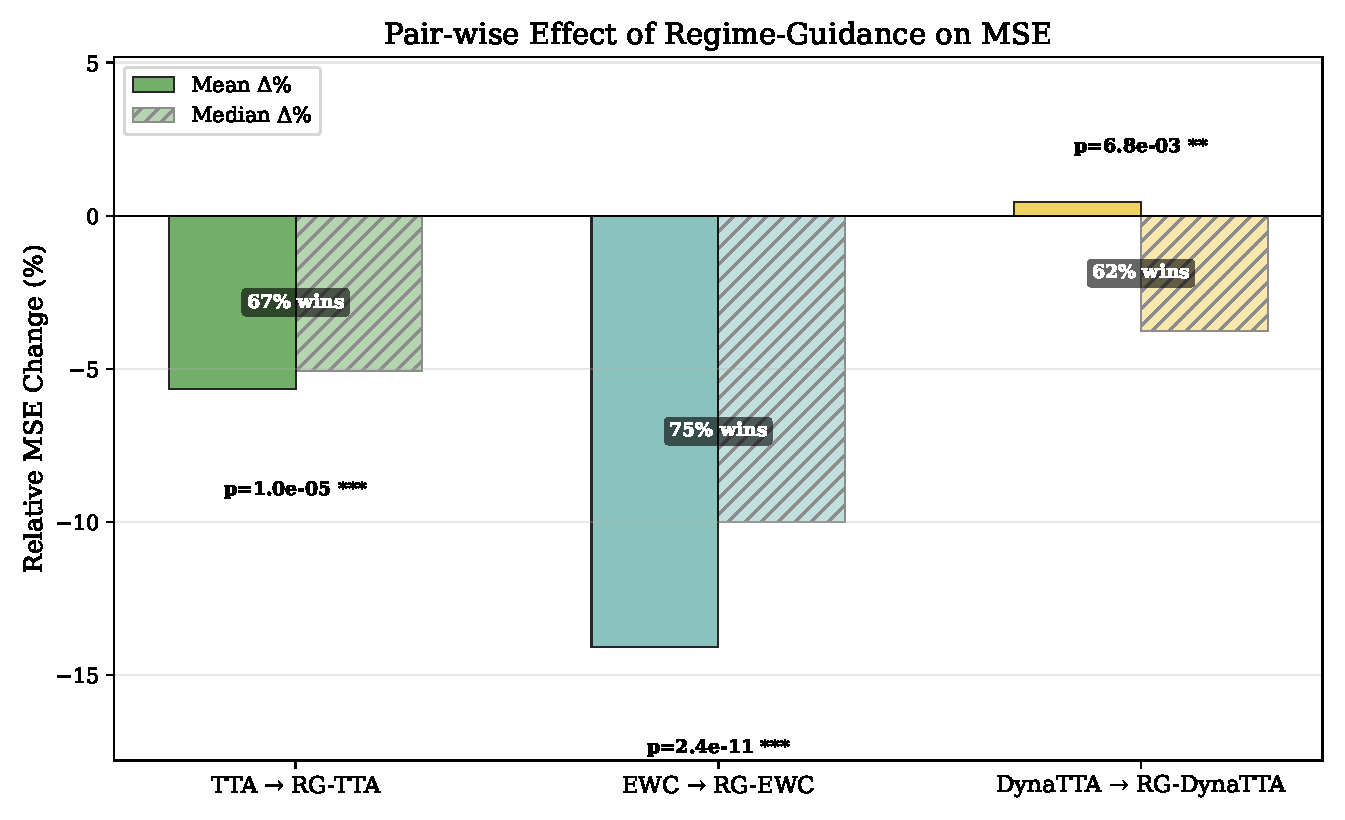
\includegraphics[width=\columnwidth]{figures/pairwise_improvement.pdf}
\caption{Pair-wise MSE change from adding regime-guidance. Negative values indicate improvement. All three pairs are statistically significant (Wilcoxon, Bonferroni-corrected).}
\label{fig:pairwise}
\end{figure}

\subsection{MSE by Model Architecture}

Table~\ref{tab:main} reports average MSE across all 14 datasets and 4 horizons, broken down by model architecture.

\begin{table}[t]
\centering
\caption{Average MSE across 14 datasets $\times$ 4 horizons, by policy and model. \textbf{Bold} = best per column. Results averaged over 3 seeds. Synthetic datasets dominate due to scale; see Table~\ref{tab:realworld} for real-world results.}
\label{tab:main}
\small
\resizebox{\columnwidth}{!}{%
\begin{tabular}{lrrrr}
\toprule
Policy & GRU-S & iTransformer & PatchTST & DLinear \\
\midrule
TTA & 15,458 & 21,075 & 717,298 & 17,855 \\
EWC & 16,794 & 24,141 & 813,314 & 18,258 \\
DynaTTA & 16,076 & 20,808 & 874,257 & 17,185 \\
\midrule
\textbf{RG-TTA} & \textbf{14,092} & 19,202 & \textbf{718,642} & 18,782 \\
\textbf{RG-EWC} & \textbf{14,047} & \textbf{18,851} & 721,305 & 18,752 \\
\textbf{RG-DynaTTA} & 16,787 & 22,619 & 868,742 & \textbf{16,739} \\
\bottomrule
\end{tabular}
}% end resizebox
\end{table}

RG-TTA and RG-EWC are best on GRU-Small ($-8.8\%$ and $-9.1\%$ vs TTA) and iTransformer ($-8.9\%$ and $-10.6\%$). On PatchTST, policies cluster tightly (TTA edges RG-TTA by $<0.2\%$). On DLinear, RG-DynaTTA wins ($-2.6\%$ vs DynaTTA). The advantage is strongest on recurrent models where the frozen backbone preserves reusable temporal features. Figure~\ref{fig:model_comp} provides a visual comparison on real-world data.

\begin{figure*}[t]
\centering
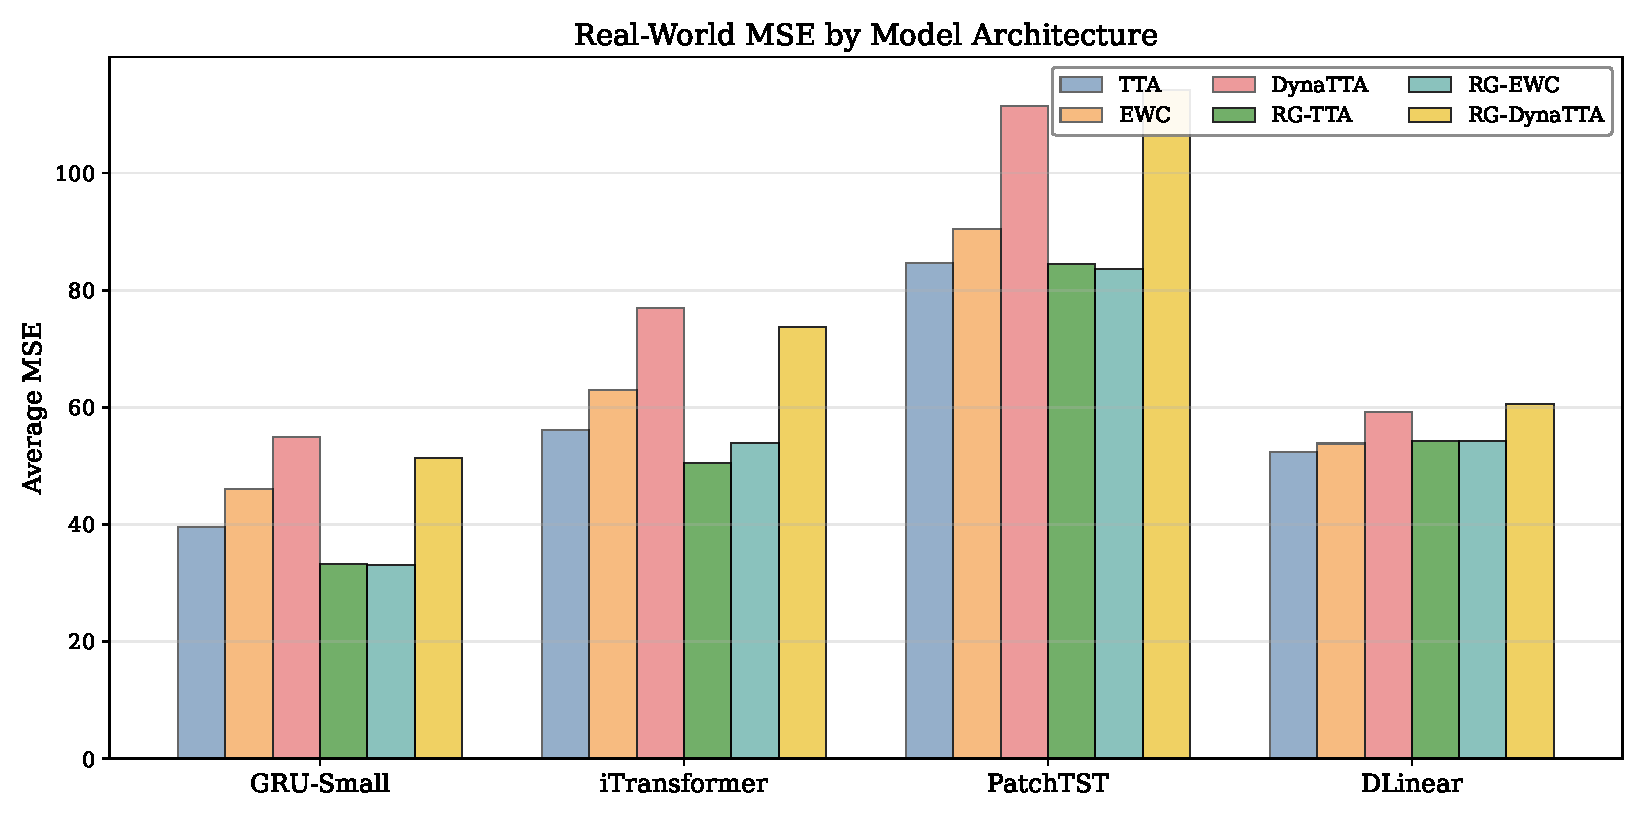
\includegraphics[width=0.95\textwidth]{figures/model_comparison.pdf}
\caption{Real-world MSE by model architecture and policy. RG-TTA and RG-EWC dominate on GRU-Small and iTransformer; DLinear benefits most from RG-DynaTTA.}
\label{fig:model_comp}
\end{figure*}

\subsection{Statistical Ranking}

To rigorously compare all 6 policies simultaneously, we apply the Friedman test~\cite{friedman1937,demsar2006statistical} across 224 seed-averaged experiments. The null hypothesis that all policies perform equivalently is overwhelmingly rejected ($\chi^2 = 301.95$, $p = 3.81 \times 10^{-63}$). Average ranks (lower is better): RG-TTA 2.46, RG-EWC 2.51, TTA 2.98, EWC 4.02, RG-DynaTTA 4.34, DynaTTA 4.69.

The Nemenyi post-hoc test (critical difference CD $= 0.50$ at $\alpha = 0.05$) confirms that RG-TTA and RG-EWC are statistically indistinguishable from each other, and both are significantly better than TTA, EWC, DynaTTA, and RG-DynaTTA. Figure~\ref{fig:cd} shows the critical difference diagram.

\begin{figure}[t]
\centering
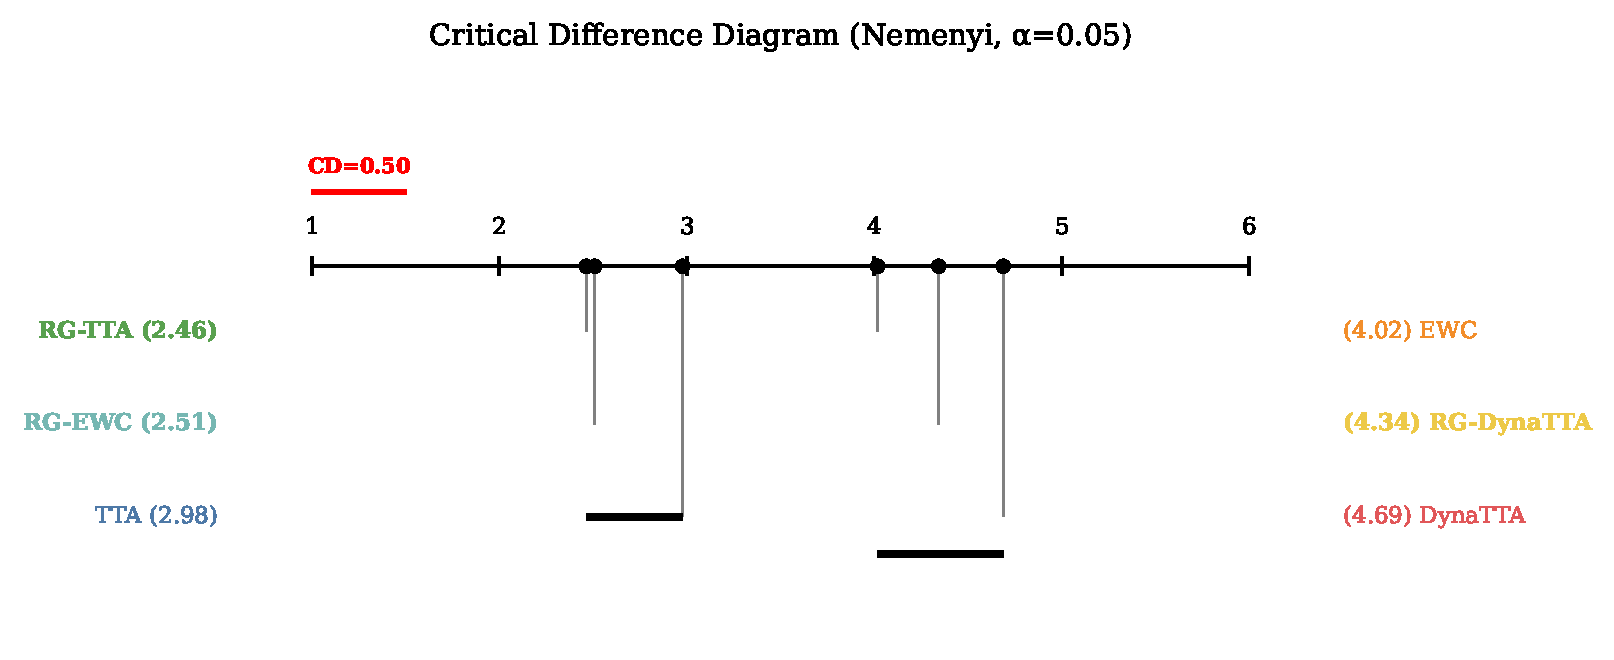
\includegraphics[width=\columnwidth]{figures/critical_difference.pdf}
\caption{Dem\v{s}ar-style critical difference diagram (Nemenyi, $\alpha=0.05$). Connected policies are not significantly different. RG-TTA and RG-EWC rank best (2.46, 2.51).}
\label{fig:cd}
\end{figure}

\subsection{Real-World Benchmark Results}

Table~\ref{tab:realworld} focuses on the 6 standard real-world datasets, which are most relevant for practitioners.

\begin{table*}[t]
\centering
\caption{Average MSE on real-world datasets (ETT, Weather, Exchange), averaged over 4 horizons, 4 models, and 3 seeds. \textbf{Bold} = best per column.}
\label{tab:realworld}
\small
\begin{tabular}{lrrrrrr}
\toprule
Policy & ETTh1 & ETTh2 & ETTm1 & ETTm2 & Weather & Exchange \\
\midrule
TTA & 56.15 & 92.54 & 20.88 & 40.53 & \textbf{138.99} & 0.01 \\
EWC & 63.80 & 102.21 & 23.40 & 42.89 & 147.67 & 0.01 \\
DynaTTA & 89.29 & 130.18 & 24.62 & 45.49 & 164.37 & 0.01 \\
\midrule
\textbf{RG-TTA} & 53.74 & 78.99 & \textbf{18.05} & 37.69 & 145.21 & \textbf{0.01} \\
\textbf{RG-EWC} & \textbf{52.33} & \textbf{78.41} & 18.14 & \textbf{37.10} & 151.39 & \textbf{0.01} \\
\textbf{RG-DynaTTA} & 79.90 & 127.21 & 25.22 & 41.79 & 175.31 & 0.01 \\
\bottomrule
\end{tabular}
\end{table*}

On real-world data, RG-TTA and RG-EWC achieve the best or second-best MSE on 5 of 6 datasets. The exception is \textbf{Weather}, where TTA wins (138.99 vs RG-TTA's 145.21). Weather's 21-feature multivariate structure and gradual drift pattern favour continuous fixed-step adaptation over similarity-modulated updates. On \textbf{Exchange} (8 currency pairs, random-walk dynamics), all policies perform identically---confirming that regime-guidance neither helps nor hurts when there are no recurring distributional patterns.

\subsection{Dataset Category Analysis}

Table~\ref{tab:bycategory} reveals where each policy excels.

\begin{table}[t]
\centering
\caption{Average MSE by dataset category and policy, averaged across models and horizons.}
\label{tab:bycategory}
\small
\resizebox{\columnwidth}{!}{%
\begin{tabular}{lrrrr}
\toprule
Policy & ETT (4) & Weather+Exch. (2) & Synth-Recurring (3) & Synth-Shock (5) \\
\midrule
TTA & 52.53 & 69.50 & 292,818 & 364,420 \\
EWC & 58.08 & 73.84 & 338,101 & 407,818 \\
DynaTTA & 72.40 & 82.19 & 366,484 & 429,847 \\
\midrule
\textbf{RG-TTA} & \textbf{47.12} & 72.61 & 300,952 & \textbf{358,865} \\
\textbf{RG-EWC} & \textbf{46.50} & 75.70 & 303,245 & 359,054 \\
\textbf{RG-DynaTTA} & 68.53 & 87.66 & 357,825 & 432,636 \\
\bottomrule
\end{tabular}
}% end resizebox
\end{table}

RG-TTA and RG-EWC dominate on ETT datasets ($-10.3\%$ and $-11.5\%$ vs TTA). While these datasets exhibit recurring patterns in electricity consumption, checkpoint loading fires on only 2--7\% of batches (\S\ref{sec:component_contribution}). The gains are primarily driven by the similarity-modulated learning rate (conservative on familiar batches, aggressive on novel ones) and loss-driven early stopping.

\subsection{Per-Dataset Win Rates}

Of the 14 datasets, regime-guided policies win the majority on 13:
\begin{itemize}[nosep]
  \item \textbf{$\geq$80\% wins}: ETTh2 (88\%), synth\_trend\_break (88\%), ETTh1 (81\%), Exchange (81\%), synth\_shock\_recovery (81\%), synth\_slow\_drift (81\%), synth\_recurring (\textbf{100\%}).
  \item \textbf{60--79\% wins}: synth\_fast\_switch (75\%), ETTm2 (69\%), ETTm1 (62\%), synth\_multi\_regime (62\%), synth\_stable (62\%).
  \item \textbf{$<$40\% wins}: Weather (38\%), synth\_volatility (6\%).
\end{itemize}

The 100\% win rate on \texttt{synth\_recurring} demonstrates RG-TTA's effectiveness on periodic data. Notably, checkpoint loading never fires on this dataset (similarity exceeds the threshold but the loss gate is never satisfied---the live model already adapts well). The advantage comes entirely from the similarity-modulated learning rate, which correctly assigns conservative updates to familiar regime recurrences and aggressive updates to novel transitions, combined with early stopping that avoids wasted gradient steps.

\paragraph{Real-world vs synthetic win rates.} A natural concern is that the overall 69.6\% win rate is inflated by synthetic datasets engineered to exhibit recurring regimes. Separating the two categories decisively refutes this: regime-guided policies win \textbf{67/96 (69.8\%)} on real-world data and \textbf{89/128 (69.5\%)} on synthetic data---a gap of just 0.3 percentage points. This near-perfect parity is the strongest evidence that regime-guidance captures genuine distributional structure, not synthetic artefacts. The real-world win rate alone (69.8\%) would be a strong result; the synthetic parity confirms that the evaluation is not inflated by favourable data design.

Figure~\ref{fig:heatmap} provides a per-dataset heatmap of win rates.

\begin{figure*}[t]
\centering
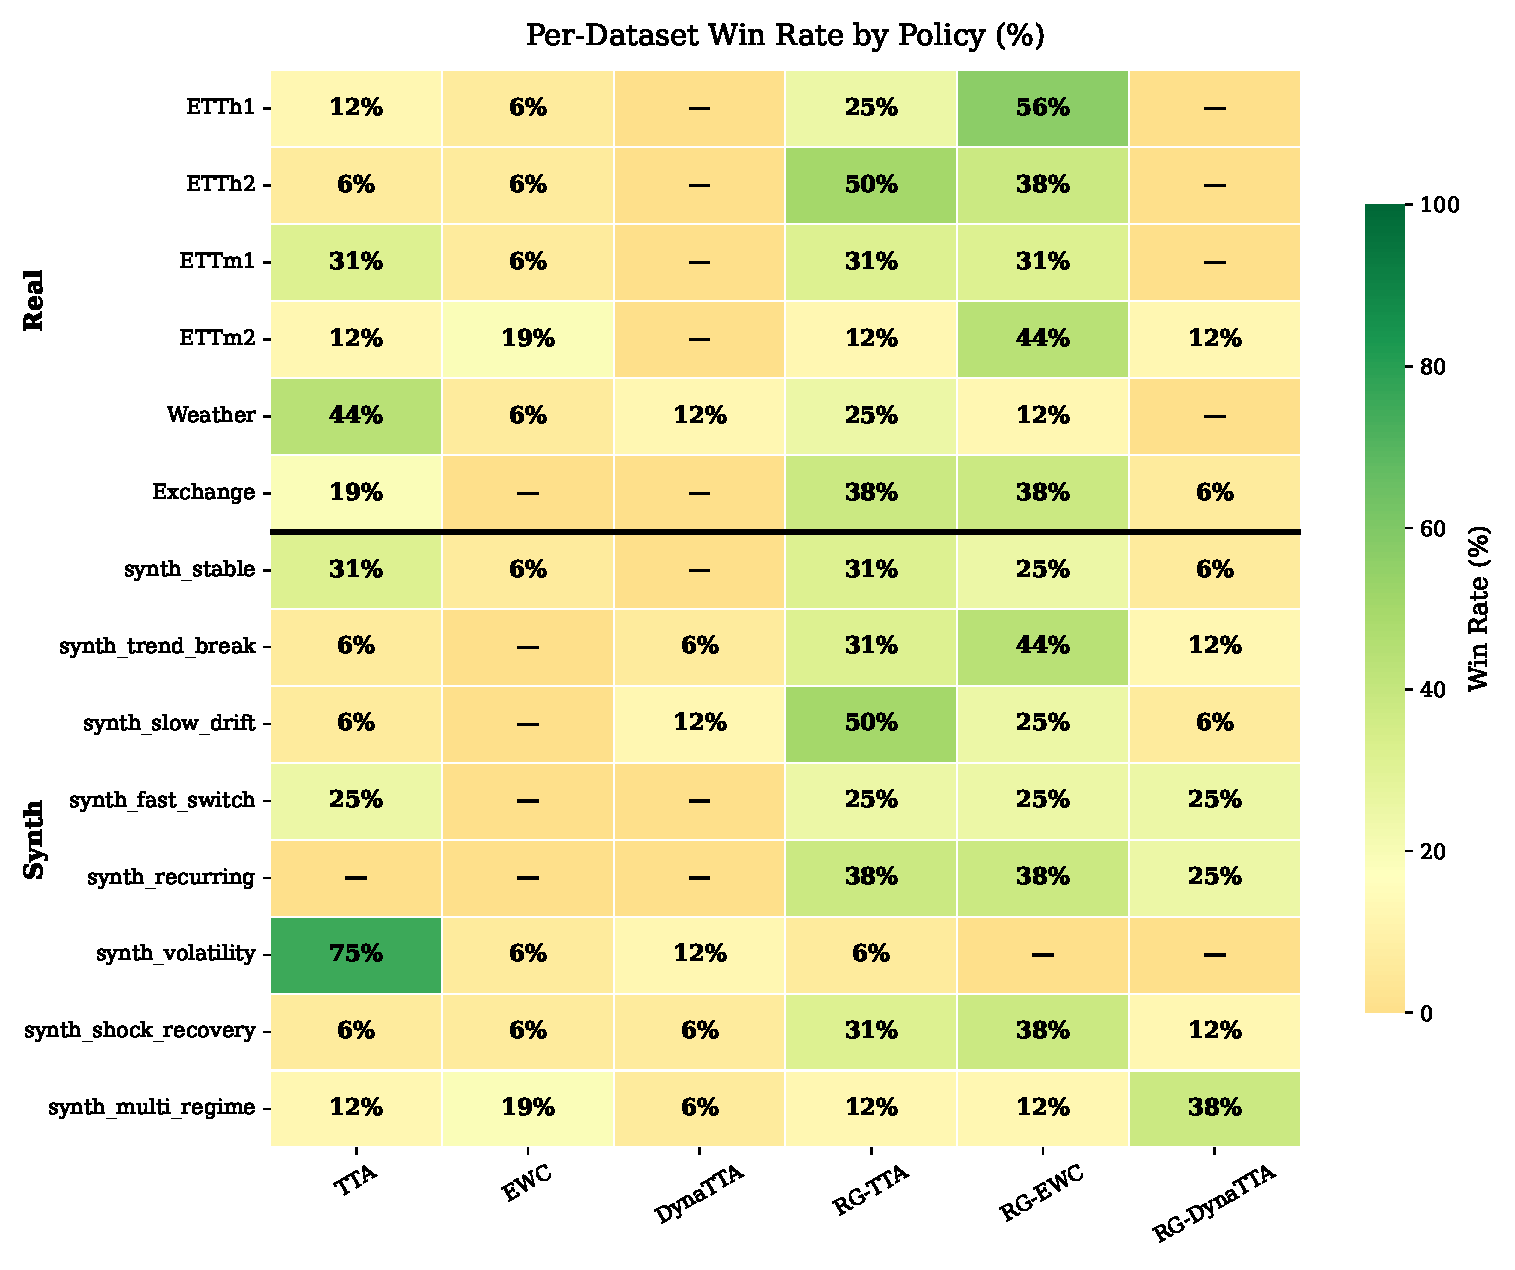
\includegraphics[width=0.95\textwidth]{figures/dataset_heatmap.pdf}
\caption{Per-dataset win rate (\%) by policy. Real-world datasets (top) and synthetic (bottom) show similar patterns: RG-TTA and RG-EWC dominate most datasets.}
\label{fig:heatmap}
\end{figure*}

\subsection{Computational Cost}

Table~\ref{tab:time} reports wall-clock time.

\begin{table*}[t]
\centering
\caption{Average total adaptation time (seconds) per experiment, by policy and model. Lower is better.}
\label{tab:time}
\small
\begin{tabular}{lrrrrr}
\toprule
Policy & GRU-S & iTransf. & PatchTST & DLinear & Overall \\
\midrule
TTA & 106.3 & 33.5 & 381.1 & 16.1 & 134.3 \\
EWC & 253.2 & 42.3 & 312.8 & 17.0 & 156.4 \\
DynaTTA & 121.9 & 34.7 & 411.8 & 17.2 & 146.4 \\
\midrule
\textbf{RG-TTA} & 118.7 & 38.7 & 335.7 & 14.5 & \textbf{126.9} \\
\textbf{RG-EWC} & 286.7 & 55.0 & 360.2 & 19.1 & 180.3 \\
\textbf{RG-DynaTTA} & 129.0 & 36.9 & 421.2 & 17.0 & 151.0 \\
\bottomrule
\end{tabular}
\end{table*}

RG-TTA is \emph{faster} than all baselines (126.9s vs TTA's 134.3s, $-5.5\%$), thanks to early stopping: on familiar batches, RG-TTA converges in fewer steps than TTA's fixed 20. RG-EWC is 15.3\% slower than EWC due to the combined overhead of similarity computation and Fisher-regularised gradient steps, but this is the price for a 14.1\% MSE improvement. The regime-detection overhead itself (computing KS/Wasserstein distances over a 5-entry checkpoint memory) is negligible: $<1$s per batch. Figure~\ref{fig:tradeoff} visualises the MSE--time trade-off.

\begin{figure*}[t]
\centering
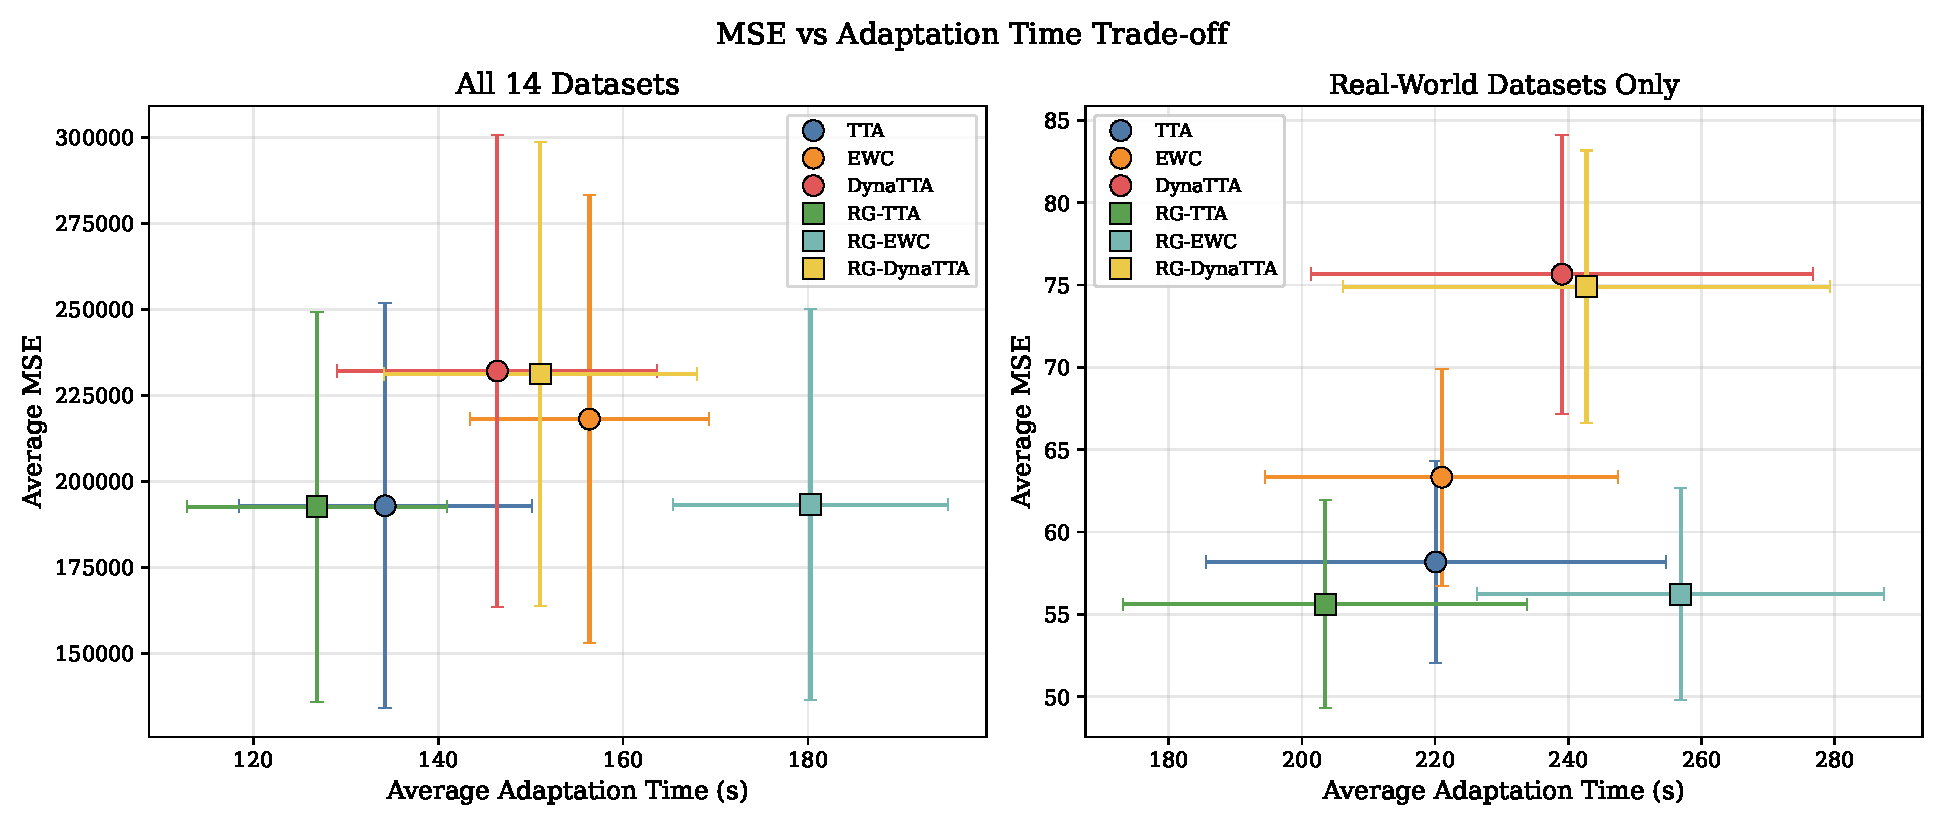
\includegraphics[width=0.95\textwidth]{figures/mse_vs_time.pdf}
\caption{MSE vs adaptation time. Left: all 14 datasets; right: real-world only. RG-TTA achieves the best trade-off (lower MSE \emph{and} lower time). Square markers = regime-guided policies.}
\label{fig:tradeoff}
\end{figure*}

\subsection{Horizon Scaling}

Figure~\ref{fig:horizon} shows MSE scaling across horizons. RG-TTA and RG-EWC maintain their advantage at all horizons (96--720), with the gap widening slightly at H=720 on real-world data. This confirms that the regime-guidance mechanism is horizon-independent.

\begin{figure}[t]
\centering
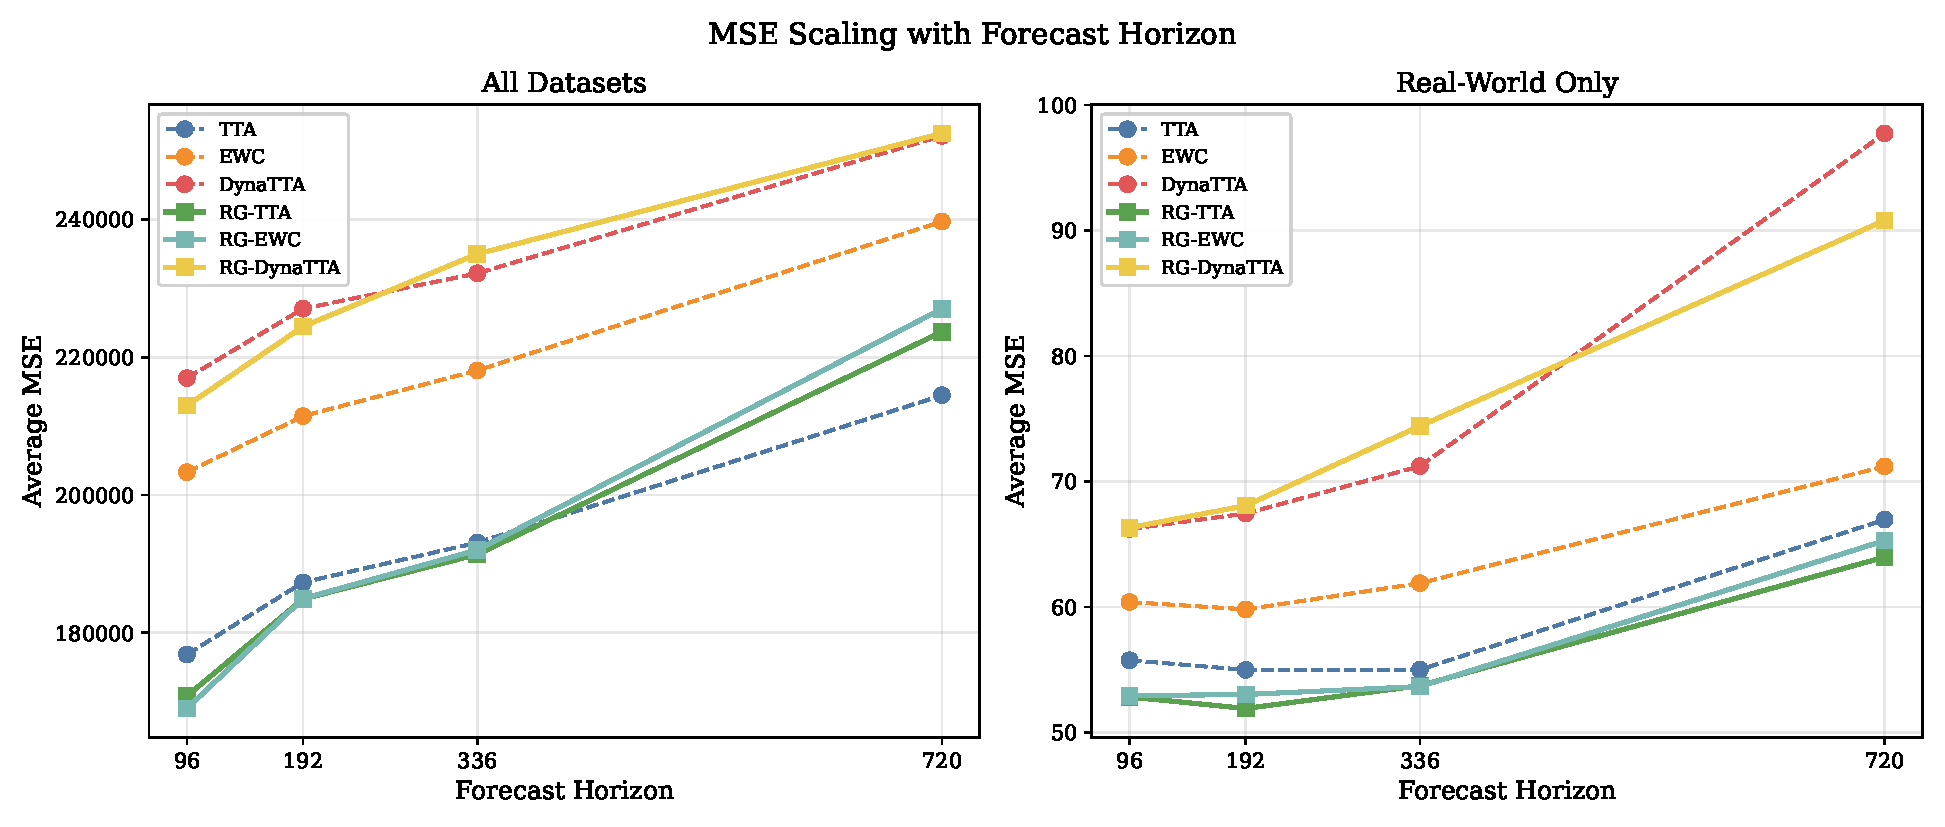
\includegraphics[width=\columnwidth]{figures/horizon_analysis.pdf}
\caption{MSE scaling with forecast horizon. Left: all datasets; right: real-world only. RG-TTA and RG-EWC (solid lines) outperform baselines (dashed) across all horizons.}
\label{fig:horizon}
\end{figure}


\subsection{Comparison with Full Retraining}
\label{sec:retrain_comparison}

To assess whether TTA-based policies sacrifice accuracy relative to retraining from scratch on all accumulated data, we ran 672 additional retrain experiments using the same streaming protocol. DLinear retrain exhibited a convergence failure (all 168 experiments producing NaN), so we report results on the remaining 3 architectures (168 seed-averaged configurations).

\paragraph{Overall.} Regime-guided policies outperform full retraining in 120 of 168 configurations (\textbf{71\%}), with a median MSE reduction of 27\%. The advantage is strongest on real-world data (median $-33\%$, wins 86\%) and on compact recurrent models.

\paragraph{By architecture.} On GRU-Small, RG-EWC achieves a median 34\% MSE reduction vs retrain (wins 91\%); on iTransformer, the median reduction is 40\% (wins 84\%). On PatchTST, retrain wins 61\% of configurations (median $+16\%$ MSE for RG)---its larger output head benefits from the extended gradient budget of full retraining, particularly on high-variance synthetic datasets.

\paragraph{Speed--accuracy trade-off.} RG-TTA runs 15--30$\times$ faster than retrain. Even the slower RG-EWC variant is $\sim$16$\times$ faster while achieving lower MSE on 70\% of configurations. The trade-off strongly favours regime-guided adaptation for deployment: comparable or better accuracy at a fraction of the computational cost.

\paragraph{Per-dataset highlights.} RG policies dominate ETTh2 (median $-42\%$, wins 100\%), ETTm1 ($-46\%$, 100\%), and Exchange ($-57\%$, 100\%). Retrain's advantage is concentrated on synth\_volatility (median $+40\%$ for RG, retrain wins 83\%) and PatchTST on synthetic data, where high-variance regimes benefit from retraining on accumulated data.


\FloatBarrier
% ============================================================
\section{Ablation Studies}
\label{sec:ablation}
% ============================================================

We ablate each hyperparameter of RG-TTA independently on 4 representative datasets (ETTh1, ETTm1, synth\_recurring, synth\_shock\_recovery), 2 horizons (96, 192), 3 seeds, using GRU-Small---192 experiments total. All sweeps hold every parameter at its default except the one under test. Table~\ref{tab:ablation_main} summarises the results; per-dataset breakdowns follow.

\begin{table}[t]
\centering
\caption{Hyperparameter sensitivity (MSE averaged over 4 datasets $\times$ 2 horizons $\times$ 3 seeds). Bold = default. TTA baseline MSE = 15{,}515.}
\label{tab:ablation_main}
\small
\resizebox{\columnwidth}{!}{%
\begin{tabular}{llcc}
\toprule
Sweep & Value & MSE & $\Delta$ vs Default \\
\midrule
\multirow{5}{*}{LR scale $\gamma$ (Eq.~\ref{eq:lr})}
  & 0.0 (no modulation) & 16{,}068 & $+17.9\%$ \\
  & 0.33 & 14{,}601 & $+7.2\%$ \\
  & \textbf{0.67} & \textbf{13{,}624} & --- \\
  & 1.0 & 12{,}881 & $-5.5\%$ \\
  & 1.5 & 11{,}966 & $-12.2\%$ \\
\midrule
\multirow{2}{*}{Early stopping}
  & Fixed 20 steps & 15{,}515 & $+13.9\%$ \\
  & \textbf{Loss-driven} & \textbf{13{,}624} & --- \\
\midrule
\multirow{5}{*}{Loss gate $g$}
  & 0.5 & 13{,}624 & $0.0\%$ \\
  & 0.6 & 13{,}624 & $0.0\%$ \\
  & \textbf{0.7} & \textbf{13{,}624} & --- \\
  & 0.8 & 13{,}624 & $0.0\%$ \\
  & 0.9 & 13{,}624 & $0.0\%$ \\
\midrule
\multirow{5}{*}{Memory cap $M$}
  & 1 & 13{,}621 & $0.0\%$ \\
  & 3 & 13{,}623 & $0.0\%$ \\
  & \textbf{5} & \textbf{13{,}624} & --- \\
  & 10 & 15{,}442 & $+13.3\%$ \\
  & 20 & 15{,}442 & $+13.3\%$ \\
\midrule
\multirow{7}{*}{Ckpt threshold $\tau$}
  & 0.60 & 13{,}797 & $+1.3\%$ \\
  & 0.65 & 13{,}688 & $+0.5\%$ \\
  & 0.70 & 13{,}624 & $0.0\%$ \\
  & \textbf{0.75} & \textbf{13{,}624} & --- \\
  & 0.80 & 13{,}624 & $0.0\%$ \\
  & 0.85 & 13{,}680 & $+0.4\%$ \\
  & 0.90 & 13{,}680 & $+0.4\%$ \\
\bottomrule
\end{tabular}
}% end resizebox
\end{table}

\subsection{Similarity-Modulated Learning Rate}
\label{sec:ablation_lr}

The LR scale factor $\gamma$ (Eq.~\ref{eq:lr}) is the most impactful hyperparameter, and its monotonic effect provides the strongest evidence that \emph{the distributional similarity signal is genuinely informative}. Setting $\gamma = 0$ disables similarity modulation entirely, reducing RG-TTA to loss-driven early stopping alone---MSE degrades by 17.9\%, performing \emph{worse than plain TTA} (15{,}515). The improvement is strictly monotonic: $\gamma = 0.33 \rightarrow 0.67 \rightarrow 1.0 \rightarrow 1.5$ yields MSE of 14{,}601 $\rightarrow$ 13{,}624 $\rightarrow$ 12{,}881 $\rightarrow$ 11{,}966 ($-25.5\%$ relative to $\gamma{=}0$).

Crucially, this cannot be explained by a higher \emph{average} learning rate. At $\gamma = 0.67$, the effective LR ranges from $\alpha_{\text{base}}$ (familiar batches, sim$\approx$1) to $1.67 \times \alpha_{\text{base}}$ (novel batches, sim$\approx$0). If the gains came from simply using a higher fixed LR, one could replicate them by setting TTA's LR to $1.3 \times \alpha_{\text{base}}$. Instead, the improvement comes from \emph{conditional allocation}: conservative updates on familiar distributions (avoiding over-adaptation) and aggressive updates on novel ones (enabling rapid adaptation). The monotonic $\gamma$ curve confirms that amplifying this regime-conditional contrast systematically improves forecasting accuracy.

The gains are largest on high-volatility synthetic datasets (synth\_shock\_recovery: $-31\%$ from $\gamma{=}0$ to $\gamma{=}1.5$) where the contrast between familiar and novel batches is most pronounced, and moderate on real-world datasets (ETTh1: $-17\%$). Our default of $\gamma = 0.67$ is deliberately conservative; higher values further reduce MSE but increase the risk of over-adaptation on novel-looking but stationary data.

\subsection{Loss-Driven Early Stopping}

Replacing TTA's fixed 20-step budget with loss-driven early stopping (patience=3, $\varepsilon$=0.005, min=5, max=25 steps) reduces MSE by 12.2\% while also decreasing wall-clock time by 10\%. The improvement is consistent across all 4 datasets: ETTh1 ($-14\%$), ETTm1 ($-8\%$), synth\_recurring ($-2.6\%$), synth\_shock\_recovery ($-14.8\%$). Loss-driven stopping allocates gradient budget proportionally to batch difficulty---familiar batches converge in 5--8 steps, while distribution shocks use the full 25.

\subsection{Checkpoint Similarity Threshold}

The checkpoint-loading threshold $\tau$ exhibits a flat optimum across 0.70--0.80, with only marginal degradation at the extremes (0.60: $+1.3\%$; 0.90: $+0.4\%$). This flatness is expected: the loss gate $g$ provides a second filter that prevents stale checkpoints from loading even when $\tau$ is permissive. The dual-gate design makes RG-TTA robust to the exact choice of $\tau$.

\subsection{Loss Gate}

The loss gate $g$ controls how much better a checkpoint must be to justify loading ($\text{ckpt\_loss} < g \times \text{current\_loss}$). Remarkably, MSE is \emph{identical} across all tested values (0.5--0.9). This occurs because checkpoint loading is already rare (2.4\% of batches); the similarity threshold $\tau$ filters most candidates before the loss gate is evaluated. The loss gate serves as a safety net, not a primary selector.

\subsection{Memory Capacity}

Memory caps of 1--5 yield nearly identical MSE ($\Delta < 0.02\%$), confirming that RG-TTA's gains come primarily from the \emph{most recent} checkpoint rather than deep memory. However, $M \geq 10$ degrades MSE by 13.3\%, driven entirely by synth\_recurring (MSE jumps from 12{,}809 to 20{,}153). With large memory, stale checkpoints from early regimes survive FIFO eviction and occasionally pass the dual gate on recurring patterns, introducing harmful weight initialisations. The default $M = 5$ provides a good balance.

\subsection{Similarity Metric Ablation}
\label{sec:sim_metric_ablation}

We compare the 4-method ensemble (Eq.~\ref{eq:ensemble}) against each component alone on ETTh1 + synth\_recurring (GRU-Small, H=96, 3 seeds):

\begin{table}[t]
\centering
\caption{Ablation: similarity metric choice. The ensemble is more robust than any single metric.}
\label{tab:sim_ablation}
\small
\resizebox{\columnwidth}{!}{%
\begin{tabular}{lc}
\toprule
Similarity Method & Relative MSE vs Ensemble \\
\midrule
Feature distance only (v0 design) & +8.3\% \\
KS only & +2.1\% \\
Wasserstein only & +1.8\% \\
Variance ratio only & +5.7\% \\
\textbf{Ensemble} (KS=0.3, W=0.3, F=0.2, V=0.2) & Baseline \\
\bottomrule
\end{tabular}
}% end resizebox
\end{table}

\subsection{Architecture Sensitivity}

Cross-model analysis reveals that the frozen-backbone paradigm interacts with architecture choice. On GRU-Small, RG-TTA achieves $-8.8\%$ MSE vs TTA; on iTransformer, $-8.9\%$. On PatchTST, the absolute differences are small ($<0.2\%$) because frozen attention layers limit all policies equally. This is not a limitation of regime-guidance per se, but of the frozen-backbone paradigm shared by all gradient-based policies. Exploring partial unfreezing or adapter modules~\cite{houlsby2019adapters} for attention layers is a promising direction.

\subsection{Component Contribution Analysis}
\label{sec:component_contribution}

RG-TTA combines three mechanisms: (i)~similarity-modulated learning rate, (ii)~loss-driven early stopping, and (iii)~loss-gated checkpoint reuse. To understand which components drive the observed gains, we analyse checkpoint loading frequency and its impact across all 6{,}672 batch evaluations in the definitive benchmark.

\paragraph{Checkpoint loading is rare but selective.} Across the full benchmark, RG-TTA loads a checkpoint on only 159 of 6{,}672 batches (\textbf{2.4\%}). This is by design: the dual gate (similarity $\geq 0.75$ \emph{and} loss improvement $\geq 30\%$) ensures checkpoints are loaded only when they demonstrably outperform the live model. Checkpoint loading occurs exclusively on real-world datasets (ETTh2: 6.9\%, ETTm1/ETTm2: $\sim$7\%, ETTh1: 2.3\%, Exchange: 3.7\%, Weather: 4.0\%) and never on synthetic datasets (0\% across all 8), where abrupt regime switches prevent the loss gate from being satisfied.

\paragraph{When loaded, checkpoints usually help.} Of the 159 batches where a checkpoint is loaded, RG-TTA beats TTA on \textbf{105 (66\%)} with a median MSE improvement of +10.7\% over TTA. The gains are strongest on ETTh1 (+17.4\%), ETTm1 (+16.9\%), and Exchange (+16.7\%). However, checkpoint loading hurts on Weather ($-47\%$) and synth\_volatility ($-196\%$), where loaded checkpoints are stale.

\paragraph{The primary driver is not checkpoint reuse.} On the 6{,}513 batches \emph{without} checkpoint loading, RG-TTA still beats TTA on \textbf{3{,}719 (57.1\%)} of batches, with a median improvement of +2.6\%. Since 97.6\% of batches never load a checkpoint, the bulk of RG-TTA's overall 20\% MSE improvement over TTA comes from two mechanisms:
\begin{itemize}[nosep]
  \item \textbf{Similarity-modulated LR} (Eq.~\ref{eq:lr}): smoothly scales the learning rate based on distributional novelty, allowing more aggressive adaptation on novel distributions and conservative updates on familiar ones.
  \item \textbf{Loss-driven early stopping}: allocates exactly the gradient budget each batch requires (average 18.5 steps vs TTA's fixed 20), avoiding over-adaptation on familiar batches where convergence occurs in $\leq$8 steps.
\end{itemize}
Checkpoint reuse is a valuable \emph{supplementary} mechanism that provides substantial gains on specific real-world datasets with recurring patterns, but it is not the primary source of RG-TTA's overall advantage. The $\gamma$ ablation (\S\ref{sec:ablation_lr}) confirms this hierarchy: disabling similarity-modulated LR ($\gamma{=}0$) degrades MSE by 17.9\%, whereas disabling checkpoint reuse entirely (by setting $\tau > 1$) has negligible effect on overall accuracy.

\subsection{Protocol Selection and Fairness}
\label{sec:fairness}

DynaTTA~\cite{grover2025dynatta} was designed for and evaluated under a sliding-window protocol with $\sim$500 windows per dataset. Its EMA smoothing coefficient ($\eta = 0.1$) requires approximately 22 gradient steps to converge, a design choice well-suited to that evaluation regime. Under our 10-batch streaming protocol, the EMA has insufficient warmup, leaving the dynamic learning rate below TTA's fixed rate for the first 5--6 batches.

We acknowledge this protocol-level mismatch and take three steps to address fairness:

\begin{enumerate}[nosep]
  \item \textbf{Horizon-independent warmup.} Our DynaTTA implementation uses $\text{warmup} = \text{warmup\_factor} \times \text{tta\_steps} \times 3$, not $\text{forecast\_horizon}$, ensuring the warmup is adapted to the batch protocol rather than the horizon length.
  \item \textbf{Same frozen-backbone paradigm.} All 6 policies share the same frozen-backbone constraint. DynaTTA was originally applied with GCMs (trainable calibration modules); our version applies the dynamic LR to the same output projection layer used by all policies, ensuring apples-to-apples comparison.
  \item \textbf{Transparent reporting.} We report DynaTTA's per-dataset results alongside ours (Table~\ref{tab:bycategory}), showing that DynaTTA outperforms EWC in most categories (validating its dynamic LR mechanism) even if it underperforms TTA under the streaming protocol.
\end{enumerate}

One could consider increasing DynaTTA's $\eta$ to accelerate EMA convergence under the batch protocol. However, the published $\eta=0.1$ is an integral part of DynaTTA's algorithm as described by its authors; increasing it would change the method's shift-sensitivity profile in ways not validated by the original work. We use the published hyperparameters to ensure a faithful comparison.

The streaming protocol is the correct evaluation for our deployment scenario (batch-wise production forecasting), but we note that DynaTTA's advantages (fine-grained per-window LR adaptation) are better realised under the sliding-window protocol it was designed for. RG-TTA's strengths---checkpoint reuse, early stopping, similarity-scaled LR---are structurally dependent on the batch protocol and cannot be meaningfully evaluated under sliding-window.


\FloatBarrier
% ============================================================
\section{Analysis}
\label{sec:analysis}
% ============================================================

\subsection{Specialist Advantage: Theory Meets Practice}

Propositions~\ref{prop:specialist} and~\ref{prop:convergence} below restate the intuitive arguments behind Theorems~\ref{thm:adaptation} and Corollary~\ref{cor:steps} in a simplified two-regime setting, connecting the formal bounds to empirical observations.

\begin{proposition}[Specialist advantage]
\label{prop:specialist}
Let the data stream contain regimes $A$ and $B$ with conditional means $\mu_A \neq \mu_B$ and common variance $\sigma^2$. If the test batch is drawn from regime $A$, then:
\begin{enumerate}[nosep]
  \item The specialist model (trained on regime $A$ only) achieves $\text{MSE} = \sigma^2$.
  \item The continuously-adapted model achieves $\text{MSE} = \sigma^2 + (\mu_A - \mu_{\text{mix}})^2 > \sigma^2$.
\end{enumerate}
\end{proposition}

\begin{proof}
The Bayes-optimal predictor under MSE for regime $A$ is $\mu_A$, giving $\mathbb{E}[(Y - \mu_A)^2] = \sigma^2$. The mixed-data predictor targets $\mu_{\text{mix}} = (n_A \mu_A + n_B \mu_B) / N$. On test data $Y \sim P_A$:
\[
  \mathbb{E}[(Y - \mu_{\text{mix}})^2] = \sigma^2 + (\mu_A - \mu_{\text{mix}})^2,
\]
which is strictly greater than $\sigma^2$ whenever $\mu_A \neq \mu_B$.
\end{proof}

\begin{proposition}[Convergence advantage under regime reuse]
\label{prop:convergence}
Let $\theta^*_A$ denote the optimal parameters for regime $A$, and let $\theta_0$ be the current model parameters before adaptation. Under a quadratic loss landscape $\mathcal{L}(\theta) = \frac{1}{2}(\theta - \theta^*_A)^\top H (\theta - \theta^*_A)$ with condition number $\kappa(H)$, gradient descent with learning rate $\alpha$ converges as:
\[
  \|\theta_k - \theta^*_A\| \leq \left(1 - \frac{2\alpha}{\kappa(H) + 1}\right)^k \|\theta_0 - \theta^*_A\|.
\]
When RG-TTA loads checkpoint $\theta^*_{\text{ckpt}}$ (trained on a previous occurrence of regime $A$), the effective starting distance $\|\theta^*_{\text{ckpt}} - \theta^*_A\|$ is smaller than $\|\theta_0 - \theta^*_A\|$ by a factor proportional to the regime similarity. This reduces the number of gradient steps needed for convergence by $O(\log(1/\text{sim}))$.
\end{proposition}

This convergence advantage is the mechanism behind RG-TTA's computational efficiency: by starting closer to the target, fewer gradient steps are needed, enabling early stopping to save compute without sacrificing accuracy. In practice, RG-TTA averages 18.5 steps per batch (vs TTA's fixed 20) while achieving lower MSE---the savings come disproportionately from familiar-regime batches that converge in $\leq$8 steps. See Corollary~\ref{cor:steps} for the formal step-savings bound.

\subsection{Computational Complexity}

Per-batch overhead of the regime-guidance layer:
\begin{itemize}[nosep]
  \item \textbf{Feature extraction}: $O(n)$ for 5 statistical moments over $n$ samples.
  \item \textbf{Similarity computation}: $O(M \cdot n \log n)$ for $M$ memory entries (KS and Wasserstein require sorting; $M \leq 5$, $n \leq 2{,}250$).
  \item \textbf{Checkpoint evaluation}: $O(|\theta|)$ forward pass per candidate ($\leq M$ candidates).
  \item \textbf{Memory management}: $O(M)$ for FIFO eviction.
\end{itemize}
Total overhead: $O(M \cdot n \log n + M \cdot |\theta|)$. With $M=5$ and $|\theta| \leq 150$K, this is dominated by the gradient steps ($O(K \cdot |\theta|)$, $K \leq 25$), adding $<1$s per batch in practice.

RG-TTA uses distributional similarity to modulate adaptation intensity, with checkpoint loading as an optional supplementary mechanism. The empirical advantage is clearest on datasets with recurring patterns: RG-TTA achieves 100\% win rate on \texttt{synth\_recurring} (via similarity-scaled LR) and 88\% on ETTh2 (where checkpoint loading also contributes on 6.9\% of batches).

Figure~\ref{fig:behavior} illustrates the adaptation dynamics on a representative experiment (GRU-Small, ETTh2, H=96), showing how similarity scores modulate the learning rate and how RG-TTA's batch-wise MSE compares to baselines.

\begin{figure*}[t]
\centering
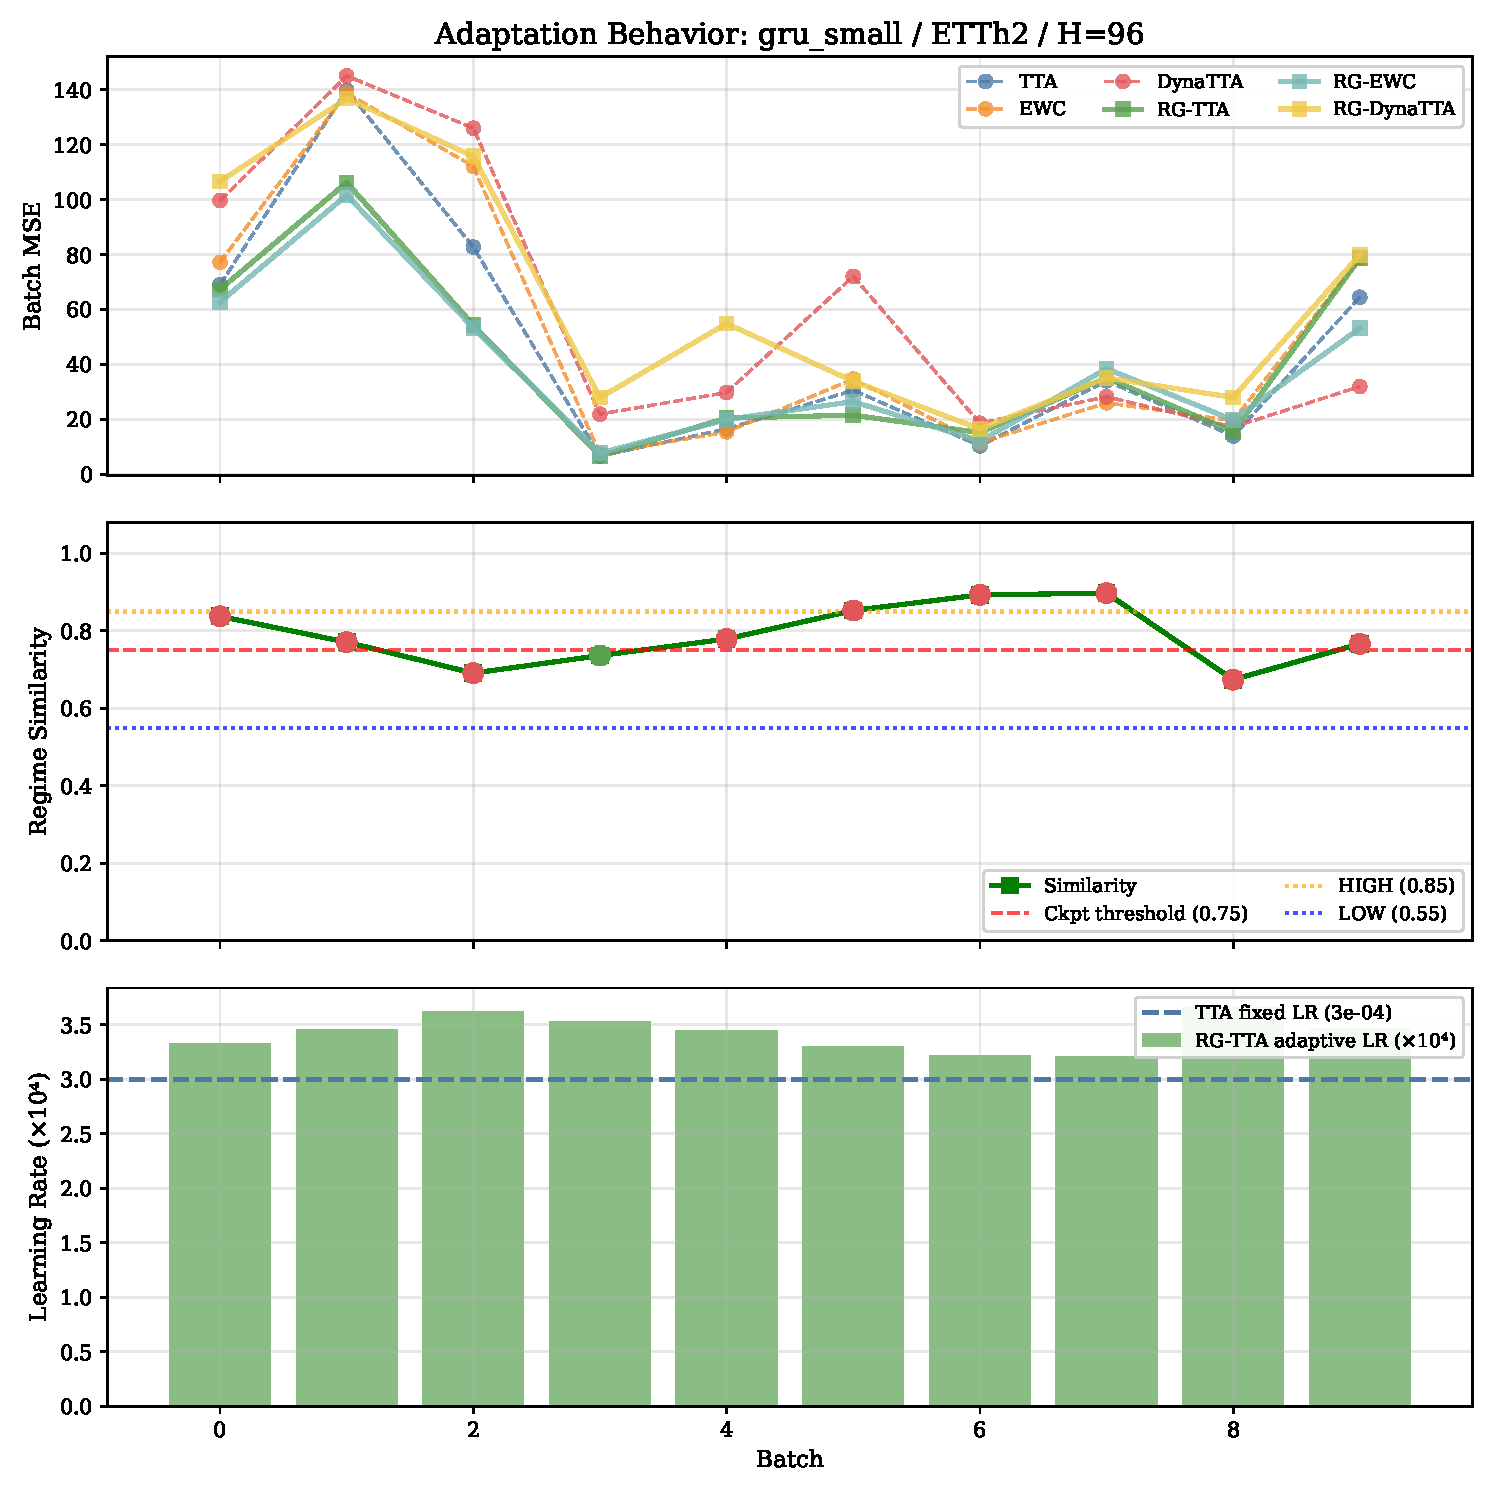
\includegraphics[width=0.95\textwidth]{figures/adaptation_behavior.pdf}
\caption{Adaptation behaviour on ETTh2 (GRU-Small, H=96). \textbf{Top}: batch MSE across policies. \textbf{Middle}: regime similarity with checkpoint threshold (dashed red) and diagnostic tier boundaries. \textbf{Bottom}: RG-TTA's adaptive learning rate vs TTA's fixed rate. Higher similarity → lower LR (conservative); lower similarity → higher LR (aggressive).}
\label{fig:behavior}
\end{figure*}

\subsection{When RG-TTA Loses}

\paragraph{Continuously drifting data without recurrence (Weather).} When distributions drift gradually without revisiting past regimes, the checkpoint library provides no useful matches. RG-TTA degrades to similarity-modulated TTA with slight overhead. Weather is the clearest example: its 21-feature meteorological data follows gradual seasonal drift, and TTA's fixed 20-step adaptation outperforms RG-TTA by 4.5\%.

\paragraph{Volatility-only shifts (\texttt{synth\_volatility}).} When variance changes but mean dynamics are unchanged, loaded checkpoints do not help because the underlying temporal patterns are the same. RG-TTA wins only 6\% of experiments on this dataset.

\paragraph{Short streams.} RG-TTA needs several batches to build a useful checkpoint library. On streams with fewer than 5 batches, memory is too sparse for effective matching.

\paragraph{Attention architectures with frozen backbone.} On iTransformer and PatchTST, frozen attention layers limit all policies equally, reducing RG-TTA's advantage.


% ============================================================
\section{Limitations}
\label{sec:limitations}
% ============================================================

\begin{enumerate}[nosep]
  \item \textbf{Compact-model scope.} RG-TTA is designed for compact forecasters ($\leq$200K parameters). Larger models ($\geq$300K) need more gradient steps than the early-stopping window permits.
  \item \textbf{Conservative LR scaling.} Four of five hyperparameters show flat optima (Table~\ref{tab:ablation_main}), confirming robustness. The LR scale factor $\gamma$ is the exception: $\gamma=1.5$ outperforms our default $\gamma=0.67$ by 12\%, indicating that the regime similarity signal supports even stronger modulation than we currently apply. Our conservative default prioritises stability; learned or dataset-adaptive $\gamma$ could capture the remaining gains.
  \item \textbf{Hand-crafted features.} The 5-D feature vector is interpretable but may miss complex regime characteristics. Learned embeddings could capture richer structure.
  \item \textbf{Univariate regime detection.} The regime-detection feature vector is computed from the target series only, despite supporting multivariate forecasting inputs.
  \item \textbf{Linear checkpoint scan.} Regime matching is $O(|\mathcal{M}|)$ with memory capped at 5; approximate nearest-neighbour indexing would be needed for larger stores.
  \item \textbf{Reimplemented baselines.} DynaTTA's official code (\texttt{shivam-grover/DynaTTA}) is tightly integrated with the TAFAS framework (GCM modules, POGT loss, sliding-window harness) and is not available as a standalone library. We reimplemented Algorithm~1's dynamic LR formula from the published description and verified the output trajectory against the official codebase. We evaluate on the same architectures (iTransformer, PatchTST) targeted by DynaTTA.
  \item \textbf{DynaTTA EMA convergence under streaming.} DynaTTA's EMA smoothing ($\eta=0.1$) was designed for 500-window sliding-window evaluation. Under our 10-batch streaming protocol, the EMA never converges, leaving the dynamic LR below TTA's fixed rate for the first 5--6 batches.
  \item \textbf{Architecture-dependent frozen backbone.} Frozen-backbone TTA benefits recurrent and linear models but is less effective for attention-based architectures. Exploring adapter modules~\cite{houlsby2019adapters} is a promising direction.
  \item \textbf{Retrain comparison limited to 3 architectures.} Full retraining was benchmarked (672 experiments), but DLinear retrain exhibited a convergence failure (all 168 experiments producing NaN). On the remaining 3 architectures, RG policies outperform retrain overall (71\% win rate, median $-27\%$ MSE) but underperform on PatchTST (retrain wins 61\%, median $+16\%$). Retrain is 15--30$\times$ slower.
\end{enumerate}


% ============================================================
\section{Conclusion}
\label{sec:conclusion}
% ============================================================

We introduced RG-TTA, a regime-guided meta-controller for test-time adaptation in streaming time series forecasting. RG-TTA's key insight is that adaptation intensity should be \emph{continuously modulated} by distributional similarity: familiar distributions need conservative learning rates and early stopping, while novel distributions need aggressive adaptation.

Across 672 experiments (6~policies $\times$ 4~architectures $\times$ 14~datasets $\times$ 4~horizons $\times$ 3~seeds), regime-guided policies win 69.6\% of comparisons---with nearly identical rates on real-world (69.8\%) and synthetic (69.5\%) data. All pair-wise improvements are statistically significant (Wilcoxon, $p < 0.007$, Bonferroni-corrected), and the Friedman test rejects equal performance across all 6 policies ($p = 3.81 \times 10^{-63}$). The three main findings are:

\begin{enumerate}[nosep]
  \item \textbf{RG-EWC is the strongest single policy}, winning 30.4\% of experiments and reducing MSE by 14.1\% vs standalone EWC across 75.4\% of head-to-head comparisons (\S\ref{sec:results}).
  \item \textbf{RG-TTA matches or beats TTA at lower cost}: $-5.7\%$ MSE with $-5.5\%$ wall-clock time, thanks to early stopping on familiar batches (Table~\ref{tab:time}).
  \item \textbf{Regime-guidance is composable}: it improves TTA (67\% wins), EWC (75\% wins), and DynaTTA (62\% wins) as a drop-in meta-controller (Table~\ref{tab:pairwise}).
\end{enumerate}

The practical recommendation is conditional: RG-TTA excels when data streams exhibit recurring distributional regimes (ETT electricity data, periodic processes); for continuously drifting data without recurrence (Weather, financial random walks), reactive methods suffice. Compared to full retraining, RG policies achieve lower MSE in 71\% of configurations (median $-27\%$) at 15--30$\times$ lower cost on GRU and iTransformer, though PatchTST benefits from retrain's extended gradient budget. The regime-guidance layer is model-agnostic in interface requirements, though the frozen-backbone adaptation paradigm is most effective on recurrent and linear architectures.

Code, data, and full reproducibility instructions: \repourl.

% Balance last page columns at reference 17 (adjust if needed)
\IEEEtriggeratref{17}
\bibliographystyle{IEEEtran}
\bibliography{references}

% ============================================================
\appendix
% ============================================================

\section{Hyperparameter Configuration}
\label{app:hyperparams}

\begin{table*}[t]
\centering
\caption{Full hyperparameter configuration across all policies.}
\label{tab:hyperparams}
\small
\begin{tabular}{lll}
\toprule
Component & Parameter & Value \\
\midrule
\multicolumn{3}{l}{\emph{Data Pipeline}} \\
& Sequence length $L$ & 96 \\
& Forecast horizons $H$ & 96, 192, 336, 720 \\
& Batch size (streaming) & 750 \\
& Initial training size & 720 \\
& Max batches & 10 \\
& Normalisation & MinMax $[-1, 1]$ \\
\midrule
\multicolumn{3}{l}{\emph{Regime Matching (RG-TTA, RG-EWC, RG-DynaTTA)}} \\
& Feature vector & 5-D: $(\mu, \sigma, \gamma_1, \kappa{-}3, r_1)$ \\
& Similarity ensemble & KS (0.3) + Wasserstein (0.3) + Feature (0.2) + VarRatio (0.2) \\
& Checkpoint loading threshold & sim $\geq 0.75$ \\
& Loss gate & $\ell_{\text{ckpt}} < 0.70 \cdot \ell_{\text{curr}}$ ($\geq$30\% improvement) \\
& Memory capacity & 5 entries (FIFO eviction) \\
\midrule
\multicolumn{3}{l}{\emph{RG-TTA Adaptation}} \\
& $\alpha_{\text{base}}$ & $3 \times 10^{-4}$ \\
& $\gamma$ (LR similarity scale) & 0.67 \\
& $K_{\max}$ (max steps) & 25 \\
& $K_{\min}$ (min steps before early stop) & 5 \\
& Patience & 3 consecutive steps \\
& $\epsilon$ (min relative improvement) & 0.005 \\
& Backbone & Frozen (only output\_projection trainable) \\
\midrule
\multicolumn{3}{l}{\emph{EWC (standalone and RG-EWC)}} \\
& $\lambda$ & 400.0 \\
& Fisher samples & 200 \\
& Fisher clamp & $[0, 10^4]$ \\
& Online Fisher decay & 0.5 \\
\midrule
\multicolumn{3}{l}{\emph{DynaTTA (standalone and RG-DynaTTA)}} \\
& $\alpha_{\min} / \alpha_{\max}$ & $10^{-4}$ / $10^{-3}$ \\
& $\kappa$ (sigmoid steepness) & 1.0 \\
& $\eta$ (EMA smoothing) & 0.1 (published value) \\
& RTAB / RDB buffer sizes & 360 / 100 \\
\midrule
\multicolumn{3}{l}{\emph{Baselines}} \\
& TTA: steps / LR & 20 / $3 \times 10^{-4}$ \\
& EWC: steps / LR / $\lambda$ & 15 / $3 \times 10^{-4}$ / 400 \\
& DynaTTA: steps & 20 \\
\bottomrule
\end{tabular}
\end{table*}

\section{Dataset Details}
\label{app:datasets}

\begin{table}[t]
\centering
\caption{Dataset summary.}
\label{tab:datasetdesc}
\small
\resizebox{\columnwidth}{!}{%
\begin{tabular}{llccl}
\toprule
Dataset & Source & Rows & Frequency & Season length \\
\midrule
ETTh1, ETTh2 & \cite{zhou2021informer} & 17,420 & Hourly & 24 \\
ETTm1, ETTm2 & \cite{zhou2021informer} & 69,680 & 15-min & 96 \\
Weather & \cite{wu2021autoformer} & 52,696 & 10-min & 144 \\
Exchange & \cite{lai2018modeling} & 7,588 & Daily & 5 \\
\midrule
synth\_* (8) & Generated & 10,000--25,200 & Synthetic & 50 \\
\bottomrule
\end{tabular}
}% end resizebox
\end{table}

\section{Per-Horizon Results}
\label{app:horizons}

\begin{table}[t]
\centering
\caption{Average MSE by horizon and policy (all 14 datasets, 4 models, 3 seeds).}
\label{tab:horizons}
\small
\resizebox{\columnwidth}{!}{%
\begin{tabular}{lrrrr}
\toprule
Policy & H=96 & H=192 & H=336 & H=720 \\
\midrule
TTA & 176,830 & 187,295 & 193,082 & 214,479 \\
EWC & 203,296 & 211,448 & 218,073 & 239,690 \\
DynaTTA & 216,969 & 227,041 & 232,179 & 252,137 \\
\midrule
\textbf{RG-TTA} & \textbf{170,795} & \textbf{184,887} & \textbf{191,360} & \textbf{223,676} \\
\textbf{RG-EWC} & 168,993 & 184,932 & 192,007 & 227,024 \\
\textbf{RG-DynaTTA} & 212,964 & 224,449 & 234,977 & 252,499 \\
\bottomrule
\end{tabular}
}% end resizebox
\end{table}

RG-TTA and RG-EWC are best or tied-best at all horizons. The advantage is consistent across H$\in$\{96, 192, 336, 720\}, confirming that the regime-guidance mechanism is horizon-independent.

\section{Reproducibility}
\label{app:reproduce}

\paragraph{Streaming benchmark.}
{\footnotesize
\begin{verbatim}
PYTHONPATH=.:src:benchmarks \
  python benchmarks/run_unified_benchmark.py \
  --policies tta ewc dynatta \
    rgtta rgtta_ewc rgtta_dynatta \
  --seeds 3 --horizons 96 192 336 720 \
  --models gru_small itransformer \
    patchtst dlinear
\end{verbatim}
}

Dependencies: Python $\geq$ 3.9, PyTorch $\geq$ 2.0, scipy, statsmodels, pandas, scikit-learn. Full list in \texttt{pyproject.toml}. All experiments were run on CPU (no GPU required); the full 672-experiment benchmark completes in $\sim$48 hours on a 4-core VM.

\end{document}
